\documentclass[12pt,a4paper]{amsart}
\usepackage{extsizes}
\usepackage{amsfonts}
\usepackage{amsthm}
\usepackage{amsmath}
\usepackage{amscd}
\usepackage[utf8]{inputenc}
\usepackage{t1enc}
\usepackage[mathscr]{eucal}
\usepackage{indentfirst}
\usepackage{graphicx}
\usepackage{graphics}
\usepackage{pict2e}
\usepackage{epic}
\numberwithin{equation}{section}
\usepackage[margin=2.9cm]{geometry}
\usepackage{epstopdf} 
\usepackage{verbatim}
\usepackage{braket}
\usepackage{cite}
\usepackage{float}
\usepackage{tikz}
\usepackage{mathtools}
\usepackage{caption}
\usepackage{textcomp}
\usetikzlibrary{decorations.pathmorphing}
\usetikzlibrary{patterns}
\usetikzlibrary{arrows}
\usetikzlibrary{arrows.meta}
\usetikzlibrary{backgrounds,fit,decorations.pathreplacing,calc}
\newcommand{\sinewave}[4][]{\draw[#1]  plot (\x,{#2*sin((#4*pi/180)r + 2*pi*#3*\x r)})}
\usetikzlibrary{decorations.pathmorphing}

\usepackage{algorithm, algorithmic}
\usepackage{xcolor}

\usepackage[colorlinks=true,allcolors=red]{hyperref}


\def\sectionautorefname{S}
\def\subsectionautorefname{S}
\def\subsubsectionautorefname{S}

\newcommand{\tosec}[1]{\textcolor{red}{[}\autoref{#1}\textcolor{red}{]}}

 \def\numset#1{{\\mathbb #1}}

\theoremstyle{plain}
\newtheorem{theorem}{Theorem}[section]
\newtheorem{Lemma}[theorem]{Lemma}
\newtheorem{Cor}[theorem]{Corollary}
\newtheorem{Prop}[theorem]{Proposition}

 \theoremstyle{definition}
\newtheorem{Def}[theorem]{Definition}
\newtheorem{Conj}[theorem]{Conjecture}
\newtheorem{Rem}[theorem]{Remark}
\newtheorem{?}[theorem]{Problem}
\newtheorem{Ex}[theorem]{Example}

\newcommand{\im}{\operatorname{im}}
\newcommand{\Hom}{{\rm{Hom}}}
\newcommand{\diam}{{\rm{diam}}}
\newcommand{\ovl}{\overline}
%\newcommand{\M}{\mathbb{M}}

\let\ab\allowbreak

\begin{document}

\captionsetup[figure]{labelfont={bf},name={Fig.},labelsep=period}

\title[Rare-earth quantum computing]{Rare-earth ion trap quantum computing:\\ The current state of the art}


\author[Nop, Paudyal, Smith]{Gavin N. Nop$^{1, 2}$, Durga Paudyal$^{1,3}$, Jonathan D.H. Smith$^{1,2}$}

%\address{$^{1}$Ames Laboratory}

%\address{$^{2}$Iowa State University \\ Department of Electrical and Computer Engineering}

%\address{$^{3}$Iowa State University \\ Department of Mathematics}



 \keywords{quantum computer; rare earth; ion trap; M\o lmer-S\o renson gate; quantum volume} 



\begin{abstract} \small 
In this review, we present the current state of the art for rare-earth based ion trap quantum computing, with a focus on industry applications. We give a brief, concrete description of various features of the quantum charge-coupled device: trap loading, electronic structure and qubit function, gates, error correction and benchmarking. We focus on current technologies to provide readers with a holistic picture of available techniques for the use of Ytterbium in modern ion designs.
\end{abstract}


\maketitle
\footnote[1]{Ames Laboratory, U.S. Department of Energy, Iowa State University, Ames, IA 50011, USA}
\footnote[2]{Department of Mathematics, Iowa State University, Ames IA 50011, USA}
\footnote[3]{Electrical and Computer Engineering Department, Iowa State University, Ames, IA 50011, USA}
\tableofcontents

%----------------------------------------------------------------------------------------
%	INTRODUCTION
%----------------------------------------------------------------------------------------

\newpage


\section{Introduction}

The history of the classical computer illustrates the progression from a proof of concept, using vacuum tubes, to the eventual sophistication of modern silicon architecture. We predict that quantum computation will chart a similar course, abandoning the relative simplicity of controlling quantized currents in superconducting loops with modern electronics, and arriving at a much more robust and sophisticated design.

Ionic quantum computers, though incompatible with classical circuitry, have been strong contenders for the future development of quantum computation, ever since Cirac and Zoller demonstrated a feasible method of applying arbitrary unitary matrices to linear arrays of ions. \cite{fundQuanIoni} More recently, two industry quantum computers using Ytterbium were introduced by Honeywell \cite{rareEartFund} and IonQ \cite{ionq}. Both computers use the lone outer $S$ shell electron of $Yb*+$ to encode quantum states. The IonQ team used a more direct method which placed all the $Yb^+$ ions in a line and applied individual addressment to the shared motional state to induce gates. The Honeywell computer used ion locomotion through magnetic fields in order to physically move qubits between gates. Both approaches show promise.\\
Our approach in this article is to give a picture of the different techniques posssible for $Yb^+$ quantum copmuters. We start \tosec[sec:prelim] with an overview of basic designs of traps for ion computers and basic info on the properties of $Yb$. After that, we proceed in the order in which a quantum computer could concevably operate, starting with --Here, I fill it out as I add labels to sections--

\section{Preliminaries}  \label{sec:prelim}


\section{QCCD architecture} 

Using ions for quantum computation allows simple methods of isolation from the surrounding environment, by suspension in an ion trap. Quantum charge coupled architecture utilizes electrodes along the ion trap to control their physical locations in a radio frequency (RF) or Paul trap \cite{compArchLarg}. In this trap, the RF electrodes are made of narrow metal plates, by which a negligibly small portion of light-induced flourescence (LIF) is blocked. Then, the LIF collection solid angle can be maximized. Barium ions can be trapped and laser-cooled in the RF trap with planar electrodes, and the crystallization is confirmed by the LIF spectrum \cite{ioniReviArt,miscQuanPap2}. The physical transport of ions can be realized while maintaining relative isolation, between gate applications, readouts, and initialization.
Between interactions, the ions are stored in memory regions. They are then propelled by the electrodes through the central region in order to implement the gates. Depending on the topology of the network, arbitrary pairs of qubits can be shuttled to the interaction region in any desired arrangement, without the need to deal with multiple ions passing each other. 
Complications arise for non-linear ion traps, as corners and intersections require fine-tuned electrode placement. Additionally, fields become less predictable, complicating the ion transport, as additional phases are liable to be induced during the transport. Linear ion traps avoid the complexities associated with intersections, at the cost of needing to effect a physical or logical ion swap. It is possible to implement quantum ion computers without ion transportation, by applying the swap gate to pairs of qubits to achieve a logical swap of the qubit states, or by using multi-qubit gates, with individual addressing \cite{fundQuanIoni}. However, ambient heating is complex to deal with, and the individual addressing may also become problematic.


\begin{figure}
\centering
\scalebox{0.4}{
\begin{tikzpicture}
\draw [fill=yellow] (-4.5,2) rectangle (-4,-0.5);
\draw [fill=yellow] (-4,2) rectangle (-3.5,-0.5);
\draw [fill=yellow] (-3.5,2) rectangle (-3,-0.5);
\draw [fill=yellow] (-0.5,2) rectangle (0,-0.5);
\draw [fill=yellow] (0,2) rectangle (0.5,-0.5);
\draw [fill=yellow] (0.5,2) rectangle (1,-0.5);
\draw [fill=yellow] (3.5,2) rectangle (4,-0.5);
\draw [fill=yellow] (4,2) rectangle (4.5,-0.5);
\draw [fill=yellow] (4.5,2) rectangle (5,-0.5);
\draw [fill=yellow] (7.5,2) rectangle (8,-0.5);
\draw [fill=yellow] (8,2) rectangle (8.5,-0.5);
\draw [fill=yellow] (8.5,2) rectangle (9,-0.5);
\draw [fill=yellow] (11.5,2) rectangle (12,-0.5);
\draw [fill=yellow] (12,2) rectangle (12.5,-0.5);
\draw [fill=yellow] (12.5,2) rectangle (13,-0.5);
\draw [fill=yellow] (15.5,2) rectangle (16,-0.5);
\draw [fill=yellow] (16,2) rectangle (16.5,-0.5);
\draw [fill=yellow] (16.5,2) rectangle (17,-0.5);
\draw [fill=yellow] (19.5,2) rectangle (20,-0.5);
\draw [fill=yellow] (20,2) rectangle (20.5,-0.5);
\draw [fill=yellow] (20.5,2) rectangle (21,-0.5);
\draw [fill=yellow] (23.5,2) rectangle (24,-0.5);
\draw [fill=yellow] (24,2) rectangle (24.5,-0.5);
\draw [fill=yellow] (24.5,2) rectangle (25,-0.5);
\draw [fill=orange] (-3,2) rectangle (-2.5,-0.5);
\draw [fill=orange] (-2.5,2) rectangle (-2,-0.5);
\draw [fill=orange] (-2,2) rectangle (-1.5,-0.5);
\draw [fill=orange] (-1.5,2) rectangle (-1,-0.5);
\draw [fill=orange] (-1,2) rectangle (-0.5,-0.5);
\draw [fill=orange] (21,2) rectangle (21.5,-0.5);
\draw [fill=orange] (21.5,2) rectangle (22,-0.5);
\draw [fill=orange] (22,2) rectangle (22.5,-0.5);
\draw [fill=orange] (22.5,2) rectangle (23,-0.5);
\draw [fill=orange] (23,2) rectangle (23.5,-0.5);
\draw [fill=cyan] (1,2) rectangle (1.5,-0.5);
\draw [fill=cyan] (1.5,2) rectangle (2,-0.5);
\draw [fill=cyan] (2,2) rectangle (2.5,-0.5);
\draw [fill=cyan] (2.5,2) rectangle (3,-0.5);
\draw [fill=cyan] (3,2) rectangle (3.5,-0.5);
\draw [fill=cyan] (5,2) rectangle (5.5,-0.5);
\draw [fill=cyan] (5.5,2) rectangle (6,-0.5);
\draw [fill=cyan] (6,2) rectangle (6.5,-0.5);
\draw [fill=cyan] (6.5,2) rectangle (7,-0.5);
\draw [fill=cyan] (7,2) rectangle (7.5,-0.5);
\draw [fill=cyan] (9,2) rectangle (9.5,-0.5);
\draw [fill=cyan] (9.5,2) rectangle (10,-0.5);
\draw [fill=cyan] (10,2) rectangle (10.5,-0.5);
\draw [fill=cyan] (10.5,2) rectangle (11,-0.5);
\draw [fill=cyan] (11,2) rectangle (11.5,-0.5);
\draw [fill=cyan] (13,2) rectangle (13.5,-0.5);
\draw [fill=cyan] (13.5,2) rectangle (14,-0.5);
\draw [fill=cyan] (14,2) rectangle (14.5,-0.5);
\draw [fill=cyan] (14.5,2) rectangle (15,-0.5);
\draw [fill=cyan] (15,2) rectangle (15.5,-0.5);
\draw [fill=cyan] (17,2) rectangle (17.5,-0.5);
\draw [fill=cyan] (17.5,2) rectangle (18,-0.5);
\draw [fill=cyan] (18,2) rectangle (18.5,-0.5);
\draw [fill=cyan] (18.5,2) rectangle (19,-0.5);
\draw [fill=cyan] (19,2) rectangle (19.5,-0.5);
\draw [fill=magenta] (25,2) rectangle (25.5,-0.5);
\draw [fill=magenta] (25.5,2) rectangle (26,-0.5);
\draw [fill=magenta] (26,2) rectangle (26.5,-0.5);
\draw [fill=gray] (-6,1.5) rectangle (28,1);
\draw [fill=gray] (28,0) rectangle (-6,0.5);
\draw [fill=black] (25.7,0.75) ellipse (0.25 and 0.25);
\end{tikzpicture}}
    \caption{A schematic of the Honeywell architecture. Here, electrodes are colored according to their role in the ion manipulation. The widths of the electrodes are not to scale, but pictured on the right is the loading hole. This constitutes the basic design of a linear ion trap. \cite{honeywell}}
\label{fig:honeywell2}
\end{figure}


A simple linear Paul trap lined with electrodes avoids these complications, as in Fig.~\ref{fig:honeywell2}.
Specific zones are as follows:
\begin{enumerate}
\item
Yellow designates auxilary zones for spacing ions when qubit gates are being applied;
\item
Blue designates qubit gate zones;
\item
Pink designates the loading zone, where qubits are introduced through the single hole;
\item
Orange denotes storage or memory zones;
\item
Grey denotes the RF electrodes used for the Paul trap.
\end{enumerate}
A total of 196 electrodes were used. The device was configured in a 2D arrangement with no line of sight between electrodes and ions\cite{honeywell}\cite{quanCopyCat}. Deterministic rotation of ion pairs with the electrodes eliminates the need for error-prone two-qubit logical swap gates.


The entire device is cooled to $12.6\,$K by use of a cold finger attached to liquid He \cite{honeywell}. Then, the ions in the array are cooled with the Doppler effect. Doppler cooling with lasers is essential to ion-trapping. It would require a substantial technological effort to monitor the ions during the cooling process. As a result, cooling is applied over an experimentally determined, fixed length of time, rather than attempting any measurement of the motional state of the ions. 


The qubit is embedded in the ${}^{171}\mathrm{Yb}^+$ ${}^2S_{1/2}$ hyperfine clock states
\begin{equation}\label{E:HypClkSt}
\ket{0} = \ket{J=0,m_J=0}\mbox{ and }\ket{1}=\ket{J=1,m_J=0}
\end{equation} 
with respective total angular momentum and $z$-component quantum numbers $J$ and $m_J$, to be visualized later. The ${}^{171}\mathrm{Yb}^+$ ions were sympathetically cooled with ${}^{138}\mathrm{Ba}^+$ ions. One of the first proposals for a similar setup envisaged a dual Yb-Ba system, with qubit states embedded in both atoms \cite{origQuanIoni}. The mass similarity between Ba and Yb provides effective Coulomb coupling, while the difference between the red-shifted Ba optical levels and the Yb optical levels allowed for independent addressing.


The ion trap in the Honeywell device is specified as a surface Paul trap operating with 190\,V at $43.35\,$MHz for radial containment, the ion trap frequencies for a single Yb being $2\pi\times 0.97\,$ MHz, $2\pi\times 2.7\,$MHz, and $2\pi\times 2.8\,$MHz for the $x$-, $y$-, and $z$-axes respectively. This additional constraint along the axial direction forms ion crystals of $\mathrm{Ba}^+$ and $\mathrm{Yb}^+$. The final four-ion crystal, which is used in the two-qubit gates, is $8\,\mu$m long \cite{honeywell}. 


Single-qubit gates are implemented using standard Rabi frequency methods. The Rabi frequency is the radian frequency of the Rabi cycle undergone for a given atomic transition in a given light field, the frequency of fluctuations in the populations of the two atomic levels involved in that atomic transition. It is proportional to the strength of the coupling between the light and the atomic transition, and to the amplitude of the light's electric field. Two-qubit gates are implemented using an alternating Hamiltonian implemented using bichromatic light to decouple internal electric states and vibrational states. These gates are applied to the four-ion chains composed of two Yb-Ba pairs. Measurements are undertaken using standard flourescent methods.


\section{Trap loading and frequency}


A common historical method of loading ion traps using electron bombardment of the source fails to distinguish isotopes of the source. In addition, electron bombardment can lead to charges on surrounding machinery, which must then be neutralized. Modern designs tend to favor photo-ionization. For quantum computers, surface ion traps are preferred, with the electrodes as far as possible from the ions, and no direct line of sight between electrodes and the suspended ions in order to prevent heating \cite{quanCopyCat}. This also allows addressing of the ions without heating the trap by setting the plane of operation for the lasers parallel to the trap surface and intersecting with the axis of the ion trap. This setup for ion addressing will be implicitly assumed from now on \cite{miscQuanPap2}.


For photo-ionization of the ytterbium in the Honeywell device, a dichoic source is composed of two counter-propagating beams, tuned to $369.53\,$nm and $398.91\,$nm, to illuminate a neutral Yb atom emitted from a heated Yb metal. The $398.91\,$nm light is tuned to the $S_{1/2}\leftrightarrow P_{1/2}$ transition which is ion-specific, allowing selection of the ${}^{171}\mathrm{Yb}$ neutral atoms, and the $369.53\,$nm wavelength ionizes the Yb atom. This is shown in Fig.~\ref{fig:YbPhoto1}. After that, the Yb$^+$ ion is Doppler cooled, using techniques discussed in Section~\ref{S:QubiCool} \cite{rareEartQubi}\cite{ioniYtteLoad}.

\begin{figure}
\centering
\scalebox{0.8}{
\begin{tikzpicture}

\node (v5) at (-3,-4) {};
\node [right] (v6) at (-2,-4) {\Large ${}^2S_{1/2}$};
\node (v3) at (-3,1.5) {};
\node [right] (v4) at (-2,1.5) {\Large  ${}^2P_{1/2}$};
\node (v1) at (-3,7) {};
\node [right] (v2) at (-2,7) {\Large $\ket{c}$};
\draw [ultra thick] (v1) edge (v2);
\draw [ultra thick] (v3) edge (v4);
\draw [ultra thick] (v5) edge (v6);
\draw [-triangle 60,decorate]
(v3) -- (v1) node [black,midway,xshift=-2cm] 
{\Large $369.53\,$nm};
\draw
[-triangle 60,decorate]
(v5) -- (v3) node [black,midway,xshift=-2cm] 
{\Large $398.91\,$nm};
\end{tikzpicture}}
    \caption{Pictured here are the transitions used in the photo-ionization of the desired ytterbium isotope. Two beams of light, each corresponding to one of the transition frequencies, illuminate a thermal stream of ions. Tuning guarantees that only ${}^{171}$Yb$^+$ is ionized, and then captured in the ion trap.}
\label{fig:YbPhoto1}
\end{figure}


\begin{figure}
\centering
\scalebox{1.0}{


\begin{tikzpicture}
\tikzset{snake it/.style={decorate, decoration=snake}}

\node (v4) at (-2,2) {};
\node (v5) at (-1,2) {};
\node (v2) at (-2,0) {};
\node (v3) at (-1,0) {};
\node (v8) at (-2,2.5) {};
\node (v9) at (-1,2.5) {};
\node (v16) at (-2,-0.5) {};
\node (v17) at (-1,-0.5) {};
\node (v26) at (-1.5,2) {};
\node (v27) at (-1.5,3.5) {};
\node (v1) at (-1.5,0) {};
\node (v33) at (-1.5,-1.5) {};

\tikzstyle{myedgestyle} = [-triangle 60]

\draw [snake it,myedgestyle] (-3,1.5) -- (v1);
\node (v20) at (1,0) {};
\node (v34) at (1.5,0) {};
\node (v22) at (1,-0.5) {};
\node (v23) at (2,-0.5) {};
\node (v35) at (1.5,-1.5) {};
\node (v6) at (1,2) {};
\node (v7) at (2,2) {};
\node (v28) at (1.5,2) {};
\node (v11) at (2,2.5) {};
\node (v10) at (1,2.5) {};
\node (v29) at (1.5,3.5) {};
\node (v12) at (4,2) {};
\node (v14) at (4,2.5) {};
\node (v30) at (4.5,2) {};
\node (v13) at (5,2) {};
\node (v15) at (5,2.5) {};
\node at (4,-0.5) {};
\node (v18) at (4,0) {};
\node at (4.5,0) {};
\node (v19) at (5,0) {};
\node at (5,-0.5) {};
\node (v36) at (4.5,-1.5) {};
\node (v31) at (4.5,3.5) {};
\node (v25) at (6,-1.5) {};
\draw  (v4) edge (v5);
\draw  (v6) edge (v7);
\draw  (v8) edge (v9);
\draw  (v10) edge (v11);
\draw  (v12) edge (v13);
\draw  (v14) edge (v15);
\draw  (v2) edge (v3);
\draw  (v16) edge (v17);
\draw  (v18) edge (v19);
\node (v21) at (2,0) {};

\draw  (v20) edge (v21);
\draw  (v22) edge (v23);
\draw  (-1.5,0) node (v32) {} ellipse (0.25 and 0.25);
\draw  (1.5,1) node (v37) {} ellipse (0.25 and 0.25);
\draw  (4.5,0) node (v24) {} ellipse (0.25 and 0.25);

\draw [myedgestyle, snake it] (v24) -- (v25);


\draw [dashed] (v26) edge (v27);
\draw [dashed] (v28) edge (v29);
\draw [dashed] (v30) edge (v31);
\draw [dashed] (v32) edge (v33);
\draw [dashed] (v34) edge (v35);
\draw [dashed] (v24) edge (v36);


\draw [myedgestyle] (v32) edge (v37);
\draw [myedgestyle] (v37) edge (v24);
\end{tikzpicture}}
    \caption{Cooling with stimulated Raman transitions. Seen here is a sample photon scattering against a constrained atom with the motional transition states pictured. If the photon does not have sufficient energy to move the atom to another motional number, the atom interacts with the photon through a Rabi oscillation and is temporarily excited to a virtual state, namely the superposition of its motional states. The coherence time being small, the qubit eventually decays according to Bon's rule.}
\label{fig:YbPhoto}
\end{figure}

\begin{figure}
\centering
\scalebox{1.0}{


\begin{tikzpicture}[domain=0:1.2, samples=120]
\tikzset{snake it/.style={decorate, decoration=snake}}
\tikzstyle{pointer} = [-triangle 60]
\sinewave[pointer,xshift=-3cm,domain=-1:2]{1.1}{2}{0};
\sinewave[pointer,xshift=3cm,domain=1:-2]{1.1}{1}{0};
\draw  (0,0) ellipse (1 and 1);

\sinewave[pointer,yshift=-3cm,xshift=-2cm,domain=1:-2]{1.1}{1}{0};
\draw [yshift=-3cm] (0,0) node (v13) {} ellipse (1 and 1);

\sinewave[pointer,yshift=-6cm,xshift=-3cm,domain=2:-1]{1.1}{2}{0};
\draw [yshift=-6cm] (0,0) node (v15) {} ellipse (1 and 1);
\node (v1) at (-0.5,0.5) {};
\node (v2) at (0.5,0.5) {};
\node (v3) at (-0.5,-0.5) {};
\node (v4) at (0.5,-0.5) {};
\node (v5) at (-0.5,-2.5) {};
\node (v6) at (0.5,-2.5) {};
\node (v7) at (-0.5,-3.5) {};
\node (v8) at (0.5,-3.5) {};
\node (v9) at (-0.5,-5.5) {};
\node (v10) at (0.5,-5.5) {};
\node (v11) at (-0.5,-6.5) {};
\node (v12) at (0.5,-6.5) {};
\draw  (v1) edge (v2);
\draw  (v3) edge (v4);
\draw  (v5) edge (v6);
\draw  (v7) edge (v8);
\draw  (v9) edge (v10);
\draw  (v11) edge (v12);
\draw  (0,-0.5) ellipse (0.25 and 0.25);
\draw  (0,-2.5) ellipse (0.25 and 0.25);
\draw  (0,-6.5) ellipse (0.25 and 0.25);
\node (v14) at (2,-3) {};
\node (v16) at (4,-6) {};
\draw [pointer] (v13) edge (v14);
\draw [pointer] (v15) edge (v16);
\end{tikzpicture}}
    \caption{Here, we illustrate the Doppler cooling process, choosing our inertial frame from the particle's initial velocity. When the particle is illuminated by two beams of light which have the same frequency with regard to some outer inertial frame, a Doppler shift occurs, as the counterpropogating beam toward which the particle moves is blue-shifted. On interaction, the internal state of the particle, shown as a two level system in this diagram, is excited. After this excitation, a decay eventually occurs in which the internal electronic state drops again, emitting a beam in a random direction. The probabilistic expectation of this interaction is a decrease in the motional energy of the particle relative to the frame where the two beams have equal frequency.}
\label{fig:YbPhotkhgjo}
\end{figure}



\begin{figure}
\centering
\scalebox{1.0}{
\begin{tikzpicture}
\tikzset{snake it/.style={decorate, decoration=snake}}
\tikzstyle{pointer} = [-triangle 60]

\node (v1) at (-2,4) {};
\node (v2) at (0,4) {};
\node (v3) at (-2,-1) {};
\node (v4) at (0,-1) {};
\node (v5) at (-2,-2.5) {};
\node (v6) at (0,-2.5) {};
\node (v7) at (-2,2.5) {};
\node (v8) at (0,2.5) {};
\draw  (v1) edge (v2);
\draw  (v3) edge (v4);
\draw  (v5) edge (v6);
\node (v9) at (-1.5,-1) {};
\node (v10) at (-1,2.5) {};
\node (v11) at (-0.5,-2) {};
\draw [dashed] (v7) edge (v8);
\draw [pointer] (v9) edge (v10);
\draw [pointer] (v10) edge (v11);
\node at (0.5,-2) {$\epsilon$};
\node at (0.5,3.5) {$\Delta$};
\end{tikzpicture}}
    \caption{Here the basic process behind a stimulated Raman transition is pictured. A given quantum state is illuminated by two beams simultaneously, so that the coherence time is relatively long compared to the interactions we consider. The first arrow shows the first transition, which has a large detuning from any other quantum state, decreasing the probability of transition. The second beam is then designed to give a small $\epsilon$ detuning from a lower state. This amplifies the probability of the transition from the higher state to the lower state, and energy can be increased or decreased depending on whether the overall transition is red-detuned or blue-detuned.}
\label{fig:YbPhosrftkhgjo}
\end{figure}

For Ba, we can surmise the technical aspects of the ionization. Because of the issues with electron bombardment, photo-ionization is again assumed, specifically photo-ionization techniques which lead to the the selection of ${}^{138}$Ba. The Ba is heated, and then illuminated by a trichroic scheme. All transitions named are implicitly assumed to be from ${}^{138}$Ba. A $791\,$nm laser is resonant to the $6s^2 {}^1S_0 \leftrightarrow  6s6p {}^3P_1$ transition, which is then excited to the continuum by a laser set to either $310\,$nm or $337\,$nm. Experimentally, both were found to be effective. Finally, a laser set to $650\,$nm is tuned to the $5D_{3/2}\leftrightarrow 6P_{1/2}$ transition. This repumps electrons which decay from $6s6p {}^3P_1$ to $5D_{3/2}$, ionizing the Ba. Doppler cooling is likewise performed, as discussed in Section~\ref{S:QubiCool} \cite{ioniBariLoad}.


\begin{figure}
\centering
\scalebox{1.0}{
\begin{tikzpicture}
\node (v5) at (-3,-2.5) {};
\node [right] (v6) at (-2.5,-2.5) { $6s^2\,^1S_0$};
\node (v3) at (-3,0) {};
\node [right] (v4) at (-2.5,0) { $6s6p\,^3P_1$};
\node (v7) at (-1.5,-1.5) {};
\node [right] (v8) at (-1,-1.5) { $5s5d\,^3D_2$};
\node (v1) at (-3,4) {};
\node [right] (v2) at (-2.5,4) { $\ket{c}$};
\draw [ultra thick] (v1) edge (v2);
\draw [ultra thick] (v3) edge (v4);
\draw [ultra thick] (v5) edge (v6);
\draw[ultra thick]  (v7) edge (v8);
\draw [-triangle 60,decorate] (v3) -- (v1) node [black,midway,xshift=-2.4cm] 
{ $337\,$nm or $310\,$nm};
\draw [-triangle 60,decorate] (v5) -- (v3) node [black,midway,xshift=-2cm] 
{ $791.1\,$nm};
\draw [-triangle 60,decorate] (v8) -- (v4) node [black,midway,xshift=2.5cm] 
{ $650\,$nm};
\node (v8) at (-3,4.5) {};
\draw [-triangle 60,decorate,transform canvas={xshift=-3mm}] (v3) -- (v8);
\end{tikzpicture}}
    \caption{The ${}^{138}$Ba$^+$ photo-ionization scheme is slightly more complex than the corresponding $^{171}$Yb$^+$ scheme. In this case, electrons may be trapped in the $5s5d\,^3D_2$ state. So, an additional beam is optionally supplied to speed the ionization process. The two transitions at the top are to the continuum, at which point the atom is ionized. Either frequency is possible, and can be chosen based on convenience without particular impact on efficiency.}
\label{fig:YbPhoto}
\end{figure}

Finally, we note the RF choice for the Paul trap. A typical frequency for $^{171}$Yb$^+$ is $\Omega = 37\,$MHz, while a typical frequency for ${}^{138}$Ba$^+$ is $\Omega = 12\,$MHz. However, this discrepancy is not an issue, since Paul trap frequencies have many different regions of stability \cite{miscQuanPap3}.


\section{The qubit ${}^{171}\mathrm{Yb}^+$}



\begin{figure}
\centering
\scalebox{1.0}{
\begin{tikzpicture}

\node (v23) at (-1.5,1.5) {};
\node (v24) at (-0.5,1.5) {};
\node (v17) at (-3,2.5) {};
\node (v18) at (-2,2.5) {};
\node (v19) at (-1.5,3) {};
\node (v20) at (-0.5,3) {};
\node (v21) at (0,3.5) {};
\node (v22) at (1,3.5) {};
\node (v7) at (-1.5,9.5) {};
\node (v8) at (-0.5,9.5) {};
\node (v3) at (-1.5,10.5) {};
\node (v4) at (-0.5,10.5) {};
\node (v1) at (-3,10.5) {};
\node (v2) at (-2,10.5) {};
\node (v5) at (0,10.5) {};
\node (v6) at (1,10.5) {};
\node (v11) at (3.5,12.5) {};
\node (v12) at (4.5,12.5) {};
\node (v9) at (3.5,13.5) {};
\node (v10) at (4.5,13.5) {};
\node (v13) at (3.5,8) {};
\node (v14) at (4.5,8) {};
\node (v15) at (3.5,7) {};
\node (v16) at (4.5,7) {};
\draw [ultra thick] (v1) -- (v2);
\draw [ultra thick] (v3) -- (v4);
\draw [ultra thick] (v5) -- (v6);
\draw [ultra thick] (v7) -- (v8);
\draw [ultra thick] (v9) -- (v10);
\draw [ultra thick] (v11) -- (v12);
\draw [ultra thick] (v13) -- (v14);
\draw [ultra thick] (v15) -- (v16);
\draw [ultra thick] (v17) -- (v18);
\draw [ultra thick] (v19) -- (v20);
\draw [ultra thick] (v21) -- (v22);
\draw [ultra thick] (v23) -- (v24);
\node at (2,3) {$J=1$};
\node at (0.5,1.5) {$J=0$};
\node at (-4,11) {${}^2P_{1/2}$};
\node at (-4,4) {${}^2S_{1/2}$};
\node at (2,14) {${}^3D[3/2]_{1/2}$};
\node at (2.5,8) {${}^2D_{3/2}$};
\node at (2,10.5) {$J=1$};
\node at (0.5,9.5) {$J=0$};
\node at (-1,3.5) {$1$};
\node at (-1,2) {$0$};
\node at (5.5,13.5) {$J=0$};
\node at (5.5,12.5) {$J=1$};
\node at (5.5,8) {$J=2$};
\node at (5.5,7) {$J=1$};

\node (v25) at (-5,10.5) {};
\node (v26) at (-5,9.5) {};
\node (v31) at (7,13.5) {};
\node (v32) at (7,12.5) {};
\node (v29) at (7,8) {};
\node (v30) at (7,7) {};
\node (v27) at (3.5,3) {};
\node (v28) at (3.5,1.5) {};
\node at (5.5,2.25) {$12.64\,$GHz};
\node at (-6.5,10) {$2.11\,$GHz};
\node at (9,7.5) {$0.86\,$GHz};
\node at (9,13) {$2.21\,$GHz};
\draw [decorate, decoration={brace, amplitude=5pt}] (v26) -- (v25);
\draw [decorate, decoration={brace, amplitude=5pt}] (v27) -- (v28);
\draw [decorate, decoration={brace, amplitude=5pt}] (v29) -- (v30);
\draw [decorate, decoration={brace, amplitude=5pt}] (v31) -- (v32);
\end{tikzpicture}
}
    \caption{${}^{171}$Yb$^+$ electronic structure. Note that the $4f$ orbitals have higher energy than the states used, thereby providing some magnetic insulation. \cite{rareEartQubi}}\label{fig:rareEartQubi1}

\end{figure}


The ${}^{171}$Yb$^+$ qubit was constructed using methods first implemented by Olmschenk \textit{et al.}\cite{rareEartQubi}. The relevant large scale electronic structure is displayed in Fig.~\ref{fig:rareEartQubi1}. The qubit states are stored in the ${}^2S_{1/2}$ hyperfine levels. Due to the electronic shielding provided by the surrounding $4f$ states, these hyperfine levels are insensitive to magnetic fields, up to first order. 


In Fig.~\ref{fig:rareEartQubi1}, we visualize the full hyperfine structure of the relevant states in the case of ${}^{171}$Yb$^+$, which has a nuclear spin of $1/2$, leading to well-defined hyperfine splitting. The $\ket{0}$ state is embedded in the ground state of the ion, while the $\ket{1}$ state is embedded in the ${}^2S_{1/2}\ket{J=1,m_J=0}$ state \eqref{E:HypClkSt}. Here, the $z$-axis of quantization is provided by a homogeneous magnetic field of order $5\,$G applied at a $\pi/2$ angle to the trap axis \cite{honeywell}. 


The coherence time for ${}^{171}$Yb$^+$ has been estimated at $2.5\,$s \cite{rareEartQubi}. It was calculated by comparative analysis of two qubits, with a Rabi pulse sequence $\pi/2$ -- $\pi$ -- $\pi/2$ applied, followed by measurement, with spacing $T/2$ -- $T/2$ -- $\epsilon$ respectively before measurement, ensuring an equal test of both $\ket{0}$ and $\ket{1}$ states. After the operation, a Gaussian exponential decay was then fitted to the fidelity. Olmschenk \textit{et al.} note that with lower static mangetic fields, the coherence time is likely to be longer \cite{rareEartQubi}. 


To quantize the qubit, an almost uniform magnetic field was introduced. However, fluctuations in the field may initiate second-order Zeeman shifts, which could be minimized with either a more stable field, or with lower absolute field intensity. In the Honeywell computer, fluctuations were kept to $0.2\,$mG, several orders of magnitude smaller than the $5\,$G absolute intensity of the field.



\subsection{Qubit initialization}


The ${}^{171}$Yb$^+$ qubit initialization is achieved by optical pumping, as illustrated in Fig.~\ref{fig:rareEartQubi3}. Dotted lines denote natural lines of decay, while solid lines denote the gaps being pumped.
\begin{figure}
\centering
\scalebox{1.0}{
\begin{tikzpicture}

\node (v23) at (-2,1.5) {};
\node (v24) at (-1,1.5) {};
\node (v17) at (-4,2.5) {};
\node (v18) at (-3,2.5) {};
\node (v19) at (-2,3) {};
\node (v20) at (-1,3) {};
\node (v21) at (0,3.5) {};
\node (v22) at (1,3.5) {};
\node (v7) at (-2,9.5) {};
\node (v8) at (-1,9.5) {};
\node (v3) at (-2,10.5) {};
\node (v4) at (-1,10.5) {};
\node (v1) at (-4,10.5) {};
\node (v2) at (-3,10.5) {};
\node (v5) at (0,10.5) {};
\node (v6) at (1,10.5) {};
\node (v11) at (3.5,12.5) {};
\node (v12) at (4.5,12.5) {};
\node (v9) at (3.5,13.5) {};
\node (v10) at (4.5,13.5) {};
\node (v13) at (3.5,8) {};
\node (v14) at (4.5,8) {};
\node (v15) at (3.5,7) {};
\node (v16) at (4.5,7) {};
\draw [ultra thick] (v1) -- (v2);
\draw [ultra thick] (v3) -- (v4);
\draw [ultra thick] (v5) -- (v6);
\draw [ultra thick] (v7) -- (v8);
\draw [ultra thick] (v9) -- (v10);
\draw [ultra thick] (v11) -- (v12);
\draw [ultra thick] (v13) -- (v14);
\draw [ultra thick] (v15) -- (v16);
\draw [ultra thick] (v17) -- (v18);
\draw [ultra thick] (v19) -- (v20);
\draw [ultra thick] (v21) -- (v22);
\draw [ultra thick] (v23) -- (v24);

\node (v25) at (-3.5,2.5) {};
\node (v30) at (-1.5,3) {};
\node (v28) at (0.5,3.5) {};
\node (v35) at (-1.5,1.5) {};
\node (v26) at (-3.5,10.5) {};
\node (v27) at (-1.5,10.5) {};
\node (v29) at (0.5,10.5) {};
\node at (-1.5,9.5) {};
\node (v34) at (4,13.5) {};
\node (v32) at (4,12.5) {};
\node (v31) at (4,8) {};
\node (v33) at (4,7) {};

\draw [-triangle 60,decorate]  (v25) -- (v26);
\draw [-triangle 60,decorate]  (v25) -- (v27);
\draw [-triangle 60,decorate]  (v28) -- (v29);
\draw [-triangle 60,decorate]  (v28) -- (v27);
\draw [-triangle 60,decorate]  (v30) -- (v29);
\draw [-triangle 60,decorate]  (v30) -- (v26);
\draw [-triangle 60,decorate]  (v31) -- (v32);
\draw [-triangle 60,decorate,transform canvas={xshift=-3mm}]  (v33) -- (v34);


\draw [-triangle 60,decorate, dashed]  (v29) -- (v35);
\draw [-triangle 60,decorate, dashed]  (v27) -- (v35);
\draw [-triangle 60,decorate, dashed]  (v26) -- (v35);
\draw [-triangle 60,decorate, dashed]  (v34) -- (v25);
\draw [-triangle 60,decorate, dashed]  (v34) -- (v30);
\draw [-triangle 60,decorate, dashed]  (v34) -- (v28);
\draw [-triangle 60,decorate, dashed]  (v32) -- (v25);
\draw [-triangle 60,decorate, dashed]  (v32) -- (v30);
\draw [-triangle 60,decorate, dashed]  (v32) -- (v28);
\draw [-triangle 60,decorate, dashed]  (v32) -- (v35);
\draw [-triangle 60,decorate, dashed]  (v29) -- (v31);
\draw [-triangle 60,decorate, dashed]  (v29) -- (v33);
\draw [-triangle 60,decorate, dashed]  (v27) -- (v31);
\draw [-triangle 60,decorate, dashed]  (v27) -- (v33);
\draw [-triangle 60,decorate, dashed]  (v26) -- (v31);
\draw [-triangle 60,decorate, dashed]  (v26) -- (v33);
\node at (1.5,3) {$J=1$};
\node at (0,1.5) {$J=0$};
\node at (-4,11.5) {${}^2P_{1/2}$};
\node at (-5,3.5) {${}^2S_{1/2}$};
\node at (2,14) {${}^3D[3/2]_{1/2}$};
\node at (2.75,7) {${}^2D_{3/2}$};
\node at (-5,10.5) {$J=1$};
\node at (-2.5,9.5) {$J=0$};
\node at (-2.5,3) {$\ket{1}$};
\node at (-2.5,1.5) {$\ket{0}$};
\node at (5.5,13.5) {$J=0$};
\node at (5.5,12.5) {$J=1$};
\node at (5.5,8) {$J=2$};
\node at (5.5,7) {$J=1$};
\end{tikzpicture}}
    \caption{${}^{171}$Yb$^+$ qubit initialization by tuning the $p$ and $s$ orbitals. All other levels are for depumping. Here, solid lines represent induced transitions, while dotted lines represent spontaneous transitions. \cite{rareEartQubi}}
    \label{fig:rareEartQubi3}
\end{figure}


In the case of optical pumping for Yb, two resonances are used.
The first is a laser tuned to the ${}^2S_{1/2}\ket{J=1} \leftrightarrow {}^2P_{1/2}\ket{J=0}$ gap at $369.53\,$nm. This beam, before illuminating the ion, is passed through a $2.1\,$GHz electro-optic modulator, which is switched on during initializiation to generate a positive first-order sideband resonance with the ${}^2S_{1/2}\ket{J=1}\leftrightarrow {}^2P_{1/2}\ket{J=1}$ transition. Once an electron is pumped from $\ket{1}$ to ${}^2P_{1/2}$, it has a $1/3$ chance of falling directly to $\ket{0}$. However, it is also possible for the electron to fall to the metastable ${}^2D_{3/2}$. To combat this, an additional beam is used to illuminate the Yb at the ${}^2D_{3/2}\ket{J=2}\leftrightarrow {}^3D[3/2]_{1/2}\ket{J=1}$ transition. This is accomplished by using an electro-optic modulator at $3.07\,$GHz to produce $935.2\,$nm light. This drives the states to ${}^3D[3/2]_{1/2}$, which then rapidly decay to ${}^2S_{1/2}$. States which decay to $\ket{1}$ are rapidly repumped through the cycle. Near perfect coherence at $\ket{0}$ is achieved in less than $0.5\,\mu$s.


\subsection{Qubit readouts}

The qubit is read out through similar fluorescent techniques, pictured in Fig.~\ref{fig:rareEartQubi4}. Here, the significance of the dashed and solid lines remains the same as in Fig.~\ref{fig:rareEartQubi3}.

\begin{figure}
\centering
\scalebox{1.0}{
\begin{tikzpicture}

\node (v23) at (-1.5,1.5) {};
\node (v24) at (-0.5,1.5) {};
\node (v17) at (-3,2.5) {};
\node (v18) at (-2,2.5) {};
\node (v19) at (-1.5,3) {};
\node (v20) at (-0.5,3) {};
\node (v21) at (0,3.5) {};
\node (v22) at (1,3.5) {};
\node (v7) at (-1.5,9.5) {};
\node (v8) at (-0.5,9.5) {};
\node (v3) at (-1.5,10.5) {};
\node (v4) at (-0.5,10.5) {};
\node (v1) at (-3,10.5) {};
\node (v2) at (-2,10.5) {};
\node (v5) at (0,10.5) {};
\node (v6) at (1,10.5) {};
\node (v11) at (3.5,12.5) {};
\node (v12) at (4.5,12.5) {};
\node (v9) at (3.5,13.5) {};
\node (v10) at (4.5,13.5) {};
\node (v13) at (3.5,8) {};
\node (v14) at (4.5,8) {};
\node (v15) at (3.5,7) {};
\node (v16) at (4.5,7) {};
\draw [ultra thick] (v1) -- (v2);
\draw [ultra thick] (v3) -- (v4);
\draw [ultra thick] (v5) -- (v6);
\draw [ultra thick] (v7) -- (v8);
\draw [ultra thick] (v9) -- (v10);
\draw [ultra thick] (v11) -- (v12);
\draw [ultra thick] (v13) -- (v14);
\draw [ultra thick] (v15) -- (v16);
\draw [ultra thick] (v17) -- (v18);
\draw [ultra thick] (v19) -- (v20);
\draw [ultra thick] (v21) -- (v22);
\draw [ultra thick] (v23) -- (v24);
\node at (2,3) {$J=1$};
\node at (0.5,1.5) {$J=0$};
\node at (-4,11) {${}^2P_{1/2}$};
\node at (-4,4) {${}^2S_{1/2}$};
\node at (2,14) {${}^3D[3/2]_{1/2}$};
\node at (2.9,8) {${}^2D_{3/2}$};
\node at (1.5,10.5) {$J=1$};
\node at (0.5,9.5) {$J=0$};
\node [left] at (-1,3.5) {$\ket{1}$};
\node [left] at (-1,2) {$\ket{0}$};
\node at (5.5,13.5) {$J=0$};
\node at (5.5,12.5) {$J=1$};
\node at (5.5,8) {$J=2$};
\node at (5.5,7) {$J=1$};
\node (v25) at (-2.5,2.5) {};
\node (v30) at (-1,3) {};
\node (v28) at (0.5,3.5) {};
\node (v35) at (-1,1.5) {};
\node (v26) at (-2.5,10.5) {};
\node (v27) at (-1,10.5) {};
\node (v29) at (0.5,10.5) {};
\node (v36) at (-1,9.5) {};
\node (v34) at (4,13.5) {};
\node (v32) at (4,12.5) {};
\node (v31) at (4,8) {};
\node (v33) at (4,7) {};


\draw [-triangle 60,decorate, dashed] (v36) -- (v33);
\draw [-triangle 60,decorate, dashed] (v34) -- (v25);
\draw [-triangle 60,decorate, dashed] (v34) -- (v30);
\draw [-triangle 60,decorate, dashed] (v32) -- (v28);

\draw [-triangle 60,decorate] (v25) -- (v36);
\draw [-triangle 60,decorate] (v30) -- (v36);
\draw [-triangle 60,decorate] (v28) -- (v36);
\draw [-triangle 60,decorate] (v33) -- (v34);
\end{tikzpicture}}
    \caption{${}^{171}$Yb$^+$ qubit readout. Note the similarities with Fig.~\ref{fig:rareEartQubi3}. Solid lines represent induced transitions, while the dotted lines represent spontaneous transitions. \cite{rareEartQubi}}
    \label{fig:rareEartQubi4}
\end{figure}

The procedure for fluorescence is similar to that used for state initialization. Again, $369.53\,$nm light is tuned in resonance with the ${}^2S_{1/2}\ket{J=1}\leftrightarrow {}^2P_{1/2}\ket{J=0}$ transition. This pumps the electrons in $\ket{1}$ almost exclusively, as the transition $\ket{0}\leftrightarrow {}^2P_{1/2}\ket{J=1}$ is detuned by $14.7\,$GHz. Any electrons in ${}^2D_{3/2}$ are then pumped and dropped, spraying photons. The estimated optimal detection fidelity for this technique is $0.9855$, and the demonstrated optimization yielded fidelity exceeds $0.98$.



\subsection{Qubit rotations}


The Honeywell machine used separate implementations for the $X,Y$ and $Z$ qubit rotations. The $X$ and $Y$ qubit rotations were implemented with commonly used techniques \cite{rareEartQubi}. A wave resonant with the $12.643\,$GHz ${}^2S_{1/2}$ hyperfine gap was applied. This microwave was controlled using a truncated waveguide located several centimeters away from the trap.


The $Z$ rotation is unusual by having been implemented using the computer input to control the qubit transport, using the accumulated AC Stark phase to stimulate the qubit address \cite{honeywell}. Qubit rotations are restricted to $\pi/2$ increments with a resolution of $\pi/500$.


\section{Qubit cooling}\label{S:QubiCool}


For the setup of the cooling apparatus, the Yb$^+$ ion is not cooled directly. Instead, its vibrational motion is linked to the mode of a ${}^{138}\mathrm{Ba}^+$ ion. Cooling addresses internal electron states, and the relaxation of the internal states to the ground state. As a result, direct addressal of the qubit would decrease the lifetime unless care was taken to avoid inducing hyperfine transitions. Instead, use is made of lasers that are detuned from the transitions of ${}^{171}$Yb$^+$, but tuned to certain transitions of ${}^{138}$Ba$^+$, and motional coupling reduces the temperature of the pair of ions.


The Honeywell paper does not specify whether the ${}^{138}$Ba$^+$ ion is cooled to zero-point energy. However, methods for cooling ions to zero-point energy exist using stimulated Raman transitions, to effect a more efficient version of Doppler cooling.


Doppler cooling in a single dimension for a gas involves the illumination of the gas along the dimension of its motion by two lasers opposing each other. When an atom is travelling towards one of the lasers, the light is blue-shifted relative to it. When the blue shift counters the red shift, the laser's frequency is tuned to the atomic transition. The atom absorbs the photon and recoils in the opposite of its direction of motion. When the atom re-emits the photon, it does so in a random direction. Thus the expectation of the speed of the atom is decreased. For free atoms, the lower limit of the doppler cooling is $\hbar \gamma / 2 k_B$, where $\gamma $ is the linewidth and $k_B$ is the Boltzmann constant \cite{miscQuanPap4}.


\subsection{${}^{138}\mathrm{Ba}^+$ electronic structure and cooling}


For ${}^{138}$Ba$^+$, the cooling methods are similar. In this case, sympathetic cooling is necessary, as the modes addressed are detuned from the Yb qubit. For effective cooling to take place, the mass of the target ion must be similar to that of the atom being cooled. This prohibits the use of lighter ions such as Be$^+$, for which efficient zero-point cooling has been demonstrated \cite{ioniSympCool, ioniRamaCool}.


In the case of even Ba$^+$ ions, there is no hyperfine structure. Zeeman splitting does occur, and is imposed on the ions. This corroborates the need for a magnetic field to quantize the qubit \cite{rareEartCool}. For initial cooling of the ${}^{138}$Ba$^+$ ion, typical Doppler cooling methods are used, as indicated below. Here, the ${}^6S_{1/2}$ Zeeman levels are separated by $10.97\,$MHz with a field of $3.919\,$G. Light at $493.5\,$nm resonates with the $6\,^2S_{1/2}\leftrightarrow 6\,^2P_{1/2}$, while $6\,^2P_{1/2}\leftrightarrow 5\,^2D_{3/2}$ forms a $649.9\,$nm   transition. 
The $6\,^2P_{1/2}\leftrightarrow 5\,^2D_{3/2}$ transition is illuminated through both the Doppler cooling and the stimulated Raman transition modes to depopulate the $5\,^2D_{3/2}$ level.
\begin{figure}
\centering
\scalebox{1.0}{
\begin{tikzpicture}

\node (v1) at (0,2.5) {};
\node (v2) at (1,2.5) {};
\node (v3) at (0,2) {};
\node (v3a) at (0,2.5) {};
\node (v4) at (1,2) {};
\node (v5) at (0,-1) {};
\node (v5a) at (0,-1.5) {};
\node (v6) at (1,-1) {};
\node (v7) at (0,-1.5) {};
\node (v8) at (1,-1.5) {};
\node (v9) at (2,1) {};
\node (v10) at (3,1) {};
\node (v12) at (0.5,2.5) {};
\node at (0.5,2) {};
\node at (0.5,-1) {};
\node at (0.5,-1.5) {};
\node (v11) at (2.5,1) {};
\draw [ultra thick] (v1) -- (v2);
\draw [ultra thick] (v3) -- (v4);
\draw [ultra thick] (v5) -- (v6);
\draw [ultra thick] (v7) -- (v8);
\draw [ultra thick] (v9) -- (v10);
\draw [-triangle 60,decorate]  (v5a) edge (v3a);
\draw [-triangle 60,decorate]  (v11) edge (v12);
\node at (2.6,2.5) {$m_j=1/2$};
\node at (2.6,2) {$m_j=-1/2$};
\node at (-1,3) {$6\,^2P_{1/2}$};
\node at (-1,-0.5) {$6\,^2S_{1/2}$};
\node at (2.6,-1) {$m_j=1/2$};
\node at (2.6,-1.5) {$m_j=-1/2$};
\node at (4,1) {$5\,^2D_{3/2}$};
\end{tikzpicture}}
    \caption{${}^{138}$Ba$^+$ Doppler cooling. Broadening allows indiscriminate transitions between Zeeman levels. States are prevented from being trapped in the $5\,^2D_{3/2}$ structure by the secondary stimulated transition. \cite{rareEartCool}}
    \label{fig:rareEartCool2}
\end{figure}

\begin{figure}
\centering
\scalebox{1.0}{
\begin{tikzpicture}

\node (v1) at (0,2.5) {};
\node (v2) at (1,2.5) {};
\node (v3) at (0,2) {};
\node (v4) at (1,2) {};
\node (v5) at (0,-1) {};
\node (v6) at (1,-1) {};
\node (v7) at (0,-1.5) {};
\node (v8) at (1,-1.5) {};
\node (v9) at (2,1) {};
\node (v10) at (3,1) {};
\node (v12) at (0.5,2.5) {};
\node at (0.5,2) {};
\node at (0.5,-1) {};
\node at (0.5,-1.5) {};
\node (v11) at (2.5,1) {};
\draw [ultra thick] (v1) -- (v2);
\draw [ultra thick] (v3) -- (v4);
\draw [ultra thick] (v5) -- (v6);
\draw [ultra thick] (v7) -- (v8);
\draw [ultra thick] (v9) -- (v10);
\draw [-triangle 60,decorate]  (v11) edge (v12);
\node at (-1,2.5) {$m_j=1/2$};
\node at (-1,2) {$m_j=-1/2$};
\node at (1.5,3) {$6\,^2P_{1/2}$};
\node at (1.5,-0.5) {$6\,^2S_{1/2}$};
\node at (-1,-1) {$m_j=1/2$};
\node at (-1,-1.5) {$m_j=-1/2$};
\node at (4,1) {$5\,^2D_{3/2}$};
\node (v13) at (0.5,1.5) {};
\draw  [transform canvas={scale=1.1,yshift=1mm},-triangle 60,decorate]  (v5) -- (v13);
\draw  [transform canvas={yshift=1mm},-triangle 60,decorate]  (v13) edge (v8);
\end{tikzpicture}}
    \caption{${}^{138}Ba^+$ stimulated Raman cooling. Here, the $\Delta$ discussed before is chosen to be below the $6\,^P_{1/2}$ state, with an epilson detuning between the $m_j$ Zeeman levels in the $s$ state. As with the Doppler cooling, an additional beam is needed to prevent trapping, and to allow the cooling cycle to continue.\cite{rareEartCool}}
    \label{fig:rareEartCool2}
\end{figure}
For Doppler pumping, as in Fig.~\ref{fig:rareEartCool2}, the beam is taken at $493.5\,$nm with no detuning. This is applied for $20\,$ms. No data are available for what the average motional state $\overline{n}$ is after Doppler cooling.


The Doppler cooled laser is passed through two acousto-optic modulators, which convert the frequency by $+160\,$MHz and $-80\,$MHz. The resulting Raman probe beam has a Rabi frequency of $\Omega_{\mathrm{probe}} = 2\pi \times 1.07\,$MHz, with an effective Rabi frequency of $2\pi \times 89\,$ kHz. The Raman $\sigma^+$ polarized light has a Rabi frequency of $2\pi \times 14.9\,$MHz. This provides a frequency difference slightly red-detuned to the Zeeman gap, and a gap from the $6\,^2S_{1/2}\leftrightarrow 6\,^2P_{1/2}$ electronic transition of $\Delta = 2\pi \times -79\,$MHz. The values were determined experimentally \cite{rareEartCool}.
The procedure results in the cooling of the ${}^{138}$Ba$^+$ ion to $\overline{n}=0.17$.

The magnetic field and choice of an even Ba ion in the Honeywell device provide evidence for use of the Zeeman transition. Further, the cooling time of $3$--$5\,$ms, compared to the time of $10\,$ms from \cite{rareEartCool}, which is of the same order of magnitude.



\section{Ion transportation}


The use of a linear Paul trap with electrodes simplifies the design of the quantum computer. The primary manipulations needed for full control over qubits in the trap are suspension, movement, swapping, and separation. Ion suspension is trivially provided by the Paul trap, so we will focus on movement, swapping, and separation in turn.


These operations allow sorting of the ions for gate application. In a single threaded model for sorting, the time taken is $O(n\log n)$, where $n$ is the number of elements. In the case of an ion trap, the ions may be addressed individually. Performing a classical simulation of the ion sorting procedure, and in parallel simply moving each ion to its designated position in the sorted result, the time taken for ion transport is reduced to $O(n)$, further enhancing the scaleability of the computer design.


\subsection{Qubit transport}


While adiabatic transport of qubits is possible, diabatic transport is much faster. However, qubits acquire a path- and time-dependent phase, based on the speed of transport. The DC Stark shift, which can affect internal states of the qubits, may be ignored here due to the insulation of the electronic fields in Yb.


Theoretically, the RF field containing the ions, together with the field due to the electrodes, may be approximated by a particle in a quadratic potential well for ions with low motional energy. Thus the Hamiltonian
$$H = \frac{p}{2m} + \frac{1}{2}m\omega^2 (x-s(t))^2$$
can be used to describe the motion of the ion, with $\omega$ being the harmonic frequency of the potential well formed by the electrostatic fields. Here $s(t)$ represents the center of the well as a function of time in $1D$ space, and the other variables are standard \cite{ioniTranErro}. By replacing the wavefunction $\ket{\psi}$ by a wavefunction $\ket{\chi}$ displaced by $s(t)$ with an appropriate displacement operator, the Schr{\"o}dinger equation becomes
$$i\hbar\ket{\chi} = (H_0 + \dot{s}(t)p)\ket{\chi}\,,$$
where $H_0$ gives the untranslated harmonic oscillator.


Under the assumption that the initial state of the oscillator is the ground state, so that $\ket{\psi}=\ket{0}$, we can solve the equation for the amplitude $\alpha(t)$ as 
$$
\alpha(t) = \sqrt{\frac{m\omega}{2\hbar}}(s(t)-e^{-i\omega t}\int_0^t\dot{s}(u)e^{i\omega u}du)
$$
with $\ket{\psi} = \ket{\alpha(t)}$.


The goal then is to leave the particle in the ground state, or near it. This is equivalent to minimizing 
$$
\alpha(t) - \sqrt{\frac{m\omega}{2\hbar}}s(t) = \sqrt{\frac{m\omega}{2\hbar}}e^{-i\omega t}\int_0^t\dot{s}(u)e^{i\omega u}du\,.
$$
By setting $s(t)=v$ for $t\in [0,t_T]$ and $0$ otherwise, the equation can be solved as 
$$
\frac{iv}{\omega}\left(1-e^{-i\omega t_T}\right)\sqrt{\frac{m\omega}{2\hbar}}\,,
$$
which becomes $0$ when ${\omega t_T}/{2\pi}$ is an integer.
Since the solution is oscillating, even for non-ideal motion, a simple numerical calculation shows how the ion may be easily brought back to the ground state for reasonably high ratios of $\omega$ to the transport distance of the ion \cite{ioniTranFast}.


In addition, the qubit can gain a local phase due to transport. To account for the phase shift, neglect the global phase:
$$
\alpha\ket{0}+\beta\ket{e}\rightarrow \alpha\ket{0}+\beta e^{i\phi}\ket{e}\,.
$$
Perturbation theory, utilizing a time-independent assumption, gives
$$
\phi=\frac{m^2}{\hbar}\bigg(\sum_{m\neq \ket{0}} \frac{|\bra{m}X\ket{0}|}{\hbar (\omega_{\ket{0}} - \omega_{m})} -  
\sum_{m\neq \ket{e}} \frac{|\bra{m}X\ket{e}|}{\hbar (\omega_{\ket{e}} - \omega_{m})}\bigg)\int_0^T \ddot{\alpha}(t)^2 dt \, .
$$
This is calculated and numerically held to $0$, except for gate action by the intermediary processor which controls the electrodes.


\subsection{Ion separation}


Separation of a 4-ion into a pair of 2-ions, together with the time-reversed process of combination, is accomplished with an octopolar electric field. Assume that the relevant qubits are contained by an RF-field which is symmetric in the $y,z$ coordinates. Then the goal is to use the electrodes in the QCCD architecture that line the trap to generate a potential field as illustrated in Fig.~\ref{fig:ioniTraSepa1}.
 
\begin{figure}
\centering
\scalebox{1.5}{
        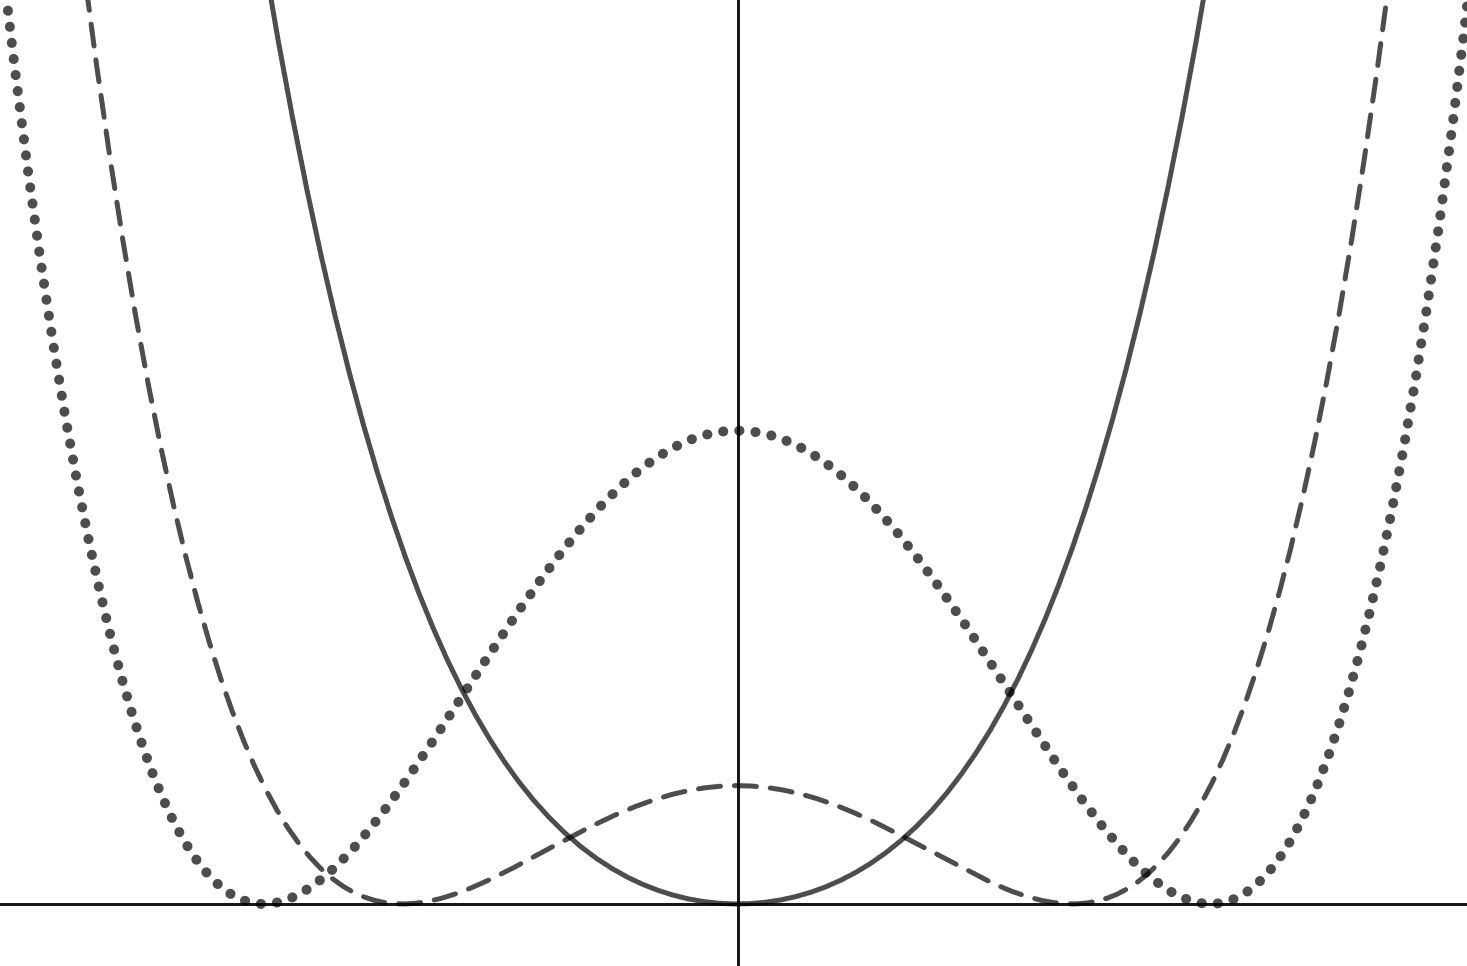
\includegraphics[totalheight=6cm]{Electrode-1.png}}
    \caption{Qubit separation potential, assumed to be symmetric. The local maximum is increased until the ions are separated. The symmetry assumption guarantees that a quartic order term alone achieves ion separation. Here, the potential for ion separation is pictured. The time sequence for the lines representing potential are in order solid, dashed, dotted. \cite{ioniTranSepa}}
    \label{fig:ioniTraSepa1}
\end{figure}

Here, the ions are at $\pm \delta$ by assumption. First, we write the potential out in terms of its Taylor expansion:
$$
V(x,0,0) = V_0 - E_0x+\alpha x^2 + E_1x^3 + \beta x^4 \,.
$$  
Then, as a simplifying assumption, we work with the case in which the electrodes are symmetric. This is motivated by noting that an asymmetric component of the separating field would merely push both ions to one side or the other of the well. Our assumption allows us to remove the cubic term. The assumption that there be two wells forces $\alpha < 0$ and $\beta > 0$. For $E_0 \sim 0$, we realize that $\partial V/\partial z = 0$ gives 
$$
s = \sqrt{\frac{|\alpha|}{2|\beta|}} \,.
$$
If we assume that $V(x,0,0)$ is constant in time, then 
$$-\alpha = \frac{m \omega_x}{4q} $$
with $\omega_x$ as the frequency of the ion.


To avoid leaking heat to the ions, the electrodes must be spaced apart from them. Now if $a$ is the minimum distance from the electrodes to the ions, we have
$$
\alpha / \beta << a^2\,.
$$
\cite{ioniTranSepa}
In fact, we take $\alpha = 0$, implying that it is possible to have an electric configuration in which the second derivative is zero and the quartic is non-zero. Laplace's equation gives $\partial^2V/\partial y^2 = -\partial^2V/\partial x^2$, implying that the field is strongly repelling in some direction in the $x$-$y$ plane. If an oscillating field is chosen, one type of Paul trap design, then the effective values of $\alpha$ and $\beta$ are reduced. Thus, it is necessary to produce an octopole. The desired potential field is
$$
V(x,y,z,t) \sim \alpha(x^2-(z^2+y^2)/2) + \beta V_4(x,y,z) + Q_{ac}cos(\Omega t)(y^2-z^2)
$$
with $V_4(x,y,z)=x^4$.


In order to achieve the required electric field configuration, at least $6$ electrodes are necessary. For an order $4$, symmetric $2$D array, the configuration in Fig.~\ref{fig:ioniTraSepa3} demonstrates an appropriate method for generating the initial octopolar moment.



\begin{figure}
\centering
\scalebox{1.0}{
\begin{tikzpicture}

\draw  (-4,2.5) rectangle (-3,1);
\draw  (-2.5,2.5) rectangle (-1.5,1);
\draw  (-1,2.5) rectangle (0,1);
\draw  (0.5,2.5) rectangle (1.5,1);
\draw  (2,2.5) rectangle (3,1);
\draw  (-4,-0.5) rectangle (-3,-2);
\draw  (-2.5,-0.5) rectangle (-1.5,-2);
\draw  (-1,-0.5) rectangle (0,-2);
\draw  (0.5,-0.5) rectangle (1.5,-2);
\draw  (2,-0.5) rectangle (3,-2);
\node at (-3.5,2) {\Huge $+$};
\node at (2.5,2) {\Huge $+$};
\node at (-3.5,-1) {\Huge $+$};
\node at (2.5,-1) {\Huge $+$};


\node at (-2,2) {\Huge $-$};
\node at (1,2) {\Huge $-$};
\node at (-2,-1) {\Huge $-$};
\node at (1,-1) {\Huge $-$};


\node at (-0.5,2) {\Large N};
\node at (-0.5,-1) {\Large N};
\end{tikzpicture}}
    \caption{An example of a linear design with the necessary quartic term. Here, the relative charges are demonstrated. These charges would occur halfway through the separation process. The two central neutral charges might also be slightly positive.}
    \label{fig:ioniTraSepa3}
\end{figure}

\subsection{Ion swapping}

Ion swapping is the process by which a string of ions is rotated about an axis orthogonal to the RF-null axis. This specific maneuver is necessary for the transport ions of between locations, as well as to maintain symmetric two-qubit gates composed of the two different ion types:
$$
\mbox{Yb--Ba--Ba--Yb\quad  and \quad Ba--Yb--Yb--Ba}\, .
$$
Although the Honetwell paper includes a complete description for a one-point and a three-point turn for the ions involved, we will visit the one-point turn in depth, and merely give a brief description of the technique behind a three-point ion turn.\cite{ioniTranSwap}


The basic configuration for the ion swapping procedure is illustrated in Fig.~\ref{fig:ioniTranSwap2}. Note the labelling in the figure. There are three configurations applied to the A,B,C,D electrodes:
\begin{enumerate}
\item electrode $x$-balance: A:\ $+$,\quad B:\ $-$,\quad C:\ $+$,\quad D:\ $-$
\item electrode $y$-balance: A:\ $-$,\quad B:\ $-$,\quad C:\ $+$,\quad D:\ $+$
\item electrode diagonal: A:\ $-$,\quad B:\ $+$,\quad C:\ $+$,\quad D:\ $-$
\end{enumerate}
In order to flip the qubit, first the side voltages are relaxed, while the endcap voltages are increased. This effectively increases the range of movement in the $x$-$y$ plane, rather than imposing linear motion.


While this happens, the primary means of controlling the direction of rotation is first applying a positive electrode diagonal, then a negative electrode diagonal as the endcap and planar electrodes are returned to their original states. This creates diagonal wells along the $y=-x$ and then along the $y=x$ directions, meaning that the ion string aligns itself $y=0$, $y=-x$, $x=0$, $y=x$, $y=0$, which completes a rotation of $\pi$. By using components of the $x$-balance and $y$-balance, a hinge in the ion string may effectively be chosen, positioning the ion chain in the $x$- and $y$-directions.
%The full electrode configuration is pictured in Fig.~\ref{fig:ioniTranSwap2}.
The relative voltage signatures and ion motions are depicted in Fig.~\ref{fig:ioniTranSwap3}.
\begin{figure}
\centering
\scalebox{1.0}{
\begin{tikzpicture}

\draw [fill=cyan] (-0.5,2) rectangle (0.5,0);
\draw  (1,2) rectangle (2,0);
\draw [fill=pink] (2.5,2) rectangle (3.5,0);
\draw  (4,2) rectangle (5,0);
\draw [fill=cyan] (5.5,2) rectangle (6.5,0);
\draw [fill=cyan] (-0.5,-3.5) rectangle (0.5,-5.5);
\draw  (1,-3.5) rectangle (2,-5.5);
\draw [fill=pink] (2.5,-3.5) rectangle (3.5,-5.5);
\draw  (4,-3.5) rectangle (5,-5.5);
\draw [fill=cyan] (5.5,-3.5) rectangle (6.5,-5.5);
\fill [red]  (-1,-0.5) rectangle (7,-1);
\fill [gray]  (-1,-1.5) rectangle (7,-2);
\fill [red]  (-1,-2.5) rectangle (7,-3);
\node (v1) at (-2,-0.5) {};
\node (v2) at (8,-0.5) {};
\node (v3) at (-2,-1) {};
\node (v4) at (8,-1) {};
\node (v5) at (-2,-1.5) {};
\node (v6) at (8,-1.5) {};
\node (v7) at (-2,-2) {};
\node (v8) at (8,-2) {};
\node (v9) at (-2,-2.5) {};
\node (v10) at (8,-2.5) {};
\node (v11) at (-2,-3) {};
\node (v12) at (8,-3) {};
\draw  (v1) edge (v2);
\draw  (v3) edge (v4);
\draw  (v5) edge (v6);
\draw  (v7) edge (v8);
\draw  (v9) edge (v10);
\draw  (v11) edge (v12);
\node at (0,1) {E};
\node at (1.5,1) {A};
\node at (3,1) {M};
\node at (4.5,1) {B};
\node at (6,1) {E};
\node at (0,-4.5) {E};
\node at (1.5,-4.5) {C};
\node at (3,-4.5) {M};
\node at (4.5,-4.5) {D};
\node at (6,-4.5) {E};
\node at (-2.5,-0.5) {RF};
\node at (-2.5,-1.5) {AE};
\node at (-2.5,-2.5) {RF};
\end{tikzpicture}}
    \caption{Electrode configuration for ion-swapping on the $x$-axis. The end cap electrodes are denoted E, Midpoint electrodes are denoted M, and the rotational electrodes are labeled A, B, C, D. The entire setup requires the crystallized ion string to be centered above the AE electrode in order to complete a rotation. The other electrodes that appear in the Honeywell architecture (\protect{Fig.~\ref{fig:honeywell2}}) serve for manipulation in the $z$- and $y$-axes.}
    \label{fig:ioniTranSwap2}
\end{figure}


\begin{figure}
\centering
\scalebox{1.0}{
\begin{tikzpicture}
\draw [ultra thick] (-5,3.5) -- (-2.5,4.5) -- (0,4.5) -- (2.5,4.5) -- (5,3.5) node (v1) {};
\draw (v1);
\draw [ultra thick]  (-5,1.5) -- (-2.5,2.5) -- (0,2.5) -- (2.5,2.5) -- (5,1.5);
\draw [ultra thick]  (-5,0.5) -- (-2.5,-0.5) -- (0,-1) -- (2.5,-0.5) -- (5,0.5);
\draw [ultra thick]  (-5,-2) -- (-2.5,-3) -- (0,-3) node (v2) {} -- (2.5,-2) -- (5,-2);
\draw [ultra thick]  (-5,-2.5) -- (-2.5,-2.5) -- (v2) -- (2.5,-3.5) -- (5,-2.5);
\draw [ultra thick]  (-5,-5.5) -- (-2.5,-4.5) -- (0,-5) node (v3) {} -- (2.5,-5.5) -- (5,-5.5);
\draw [ultra thick]  (-5,-6) -- (-2.5,-6) -- (v3) -- (2.5,-5) -- (5,-6);
\node at (-6,-6) {\Large A};
\node at (-6,-5) {\Large C};
\node at (-6,-2) {\Large D};
\node at (-6,-3) {\Large B};
\node at (-6,0) {\Large M};
\node at (-6,2) {\Large AE};
\node at (-6,4) {\Large E};
\draw  (0,-7) ellipse (0.5 and 0.5) node {\Large 2};
\draw  (0,-8) ellipse (0.5 and 0.5) node {\Large 1};
\draw  (3,-7) ellipse (0.5 and 0.5) node {\Large 2};
\draw  (2,-8) ellipse (0.5 and 0.5) node {\Large 1};
\draw  (5.5,-8) ellipse (0.5 and 0.5) node {\Large 2};
\draw  (4.5,-8) ellipse (0.5 and 0.5) node {\Large 1};
\draw  (-2,-8) ellipse (0.5 and 0.5) node {\Large 1};
\draw  (-3,-7) ellipse (0.5 and 0.5) node {\Large 2};
\draw  (-4.5,-8) ellipse (0.5 and 0.5) node {\Large 1};
\draw  (-5.5,-8) ellipse (0.5 and 0.5) node {\Large 2};
\node at (-5,6) {\Large I};
\node at (-2.5,6) {\Large II};
\node at (0,6) {\Large III};
\node at (2.5,6) {\Large IV};
\node at (5,6) {\Large V};
\node [right](v5) at (5,4.5) {55V};
\node [right](v9) at (5,3.5) {50V};
\node [right](v11) at (5,2.5) {8V};
\node [right](v15) at (5,1.5) {7.5V};
\node [right](v17) at (5,0.5) {25};
\node [right](v21) at (5,-0.5) {20V};
\node [right](v23) at (5,-1) {17.5V};
\node [right](v25) at (5,-2) {-1.5V};
\node [right](v29) at (5,-3) {-2.5V};
\node [right](v31) at (5,-3.5) {-3V};
\node [right](v27) at (5,-2.5) {-2V};
\node [right](v19) at (5,0) {22.5V};
\node [right](v13) at (5,2) {7.75V};
\node [right](v7) at (5,4) {52.5V};
\node [right](v33) at (5,-4.5) {3V};
\node [right](v35) at (5,-5) {2.5V};
\node [right](v37) at (5,-5.5) {2V};
\node [right](v39) at (5,-6) {1.5V};
\node (v4) at (-5,4.5) {};
\node (v6) at (-5,4) {};
\node (v8) at (-5,3.5) {};
\node (v10) at (-5,2.5) {};
\node (v12) at (-5,2) {};
\node (v14) at (-5,1.5) {};
\node (v16) at (-5,0.5) {};
\node (v18) at (-5,0) {};
\node (v20) at (-5,-0.5) {};
\node (v22) at (-5,-1) {};
\node (v24) at (-5,-2) {};
\node (v26) at (-5,-2.5) {};
\node (v28) at (-5,-3) {};
\node (v30) at (-5,-3.5) {};
\node (v32) at (-5,-4.5) {};
\node (v34) at (-5,-5) {};
\node (v36) at (-5,-5.5) {};
\node (v38) at (-5,-6) {};
\draw [very thin]  (v4) edge (v5);
\draw [very thin]  (v6) edge (v7);
\draw [very thin]  (v8) edge (v9);
\draw [very thin]  (v10) edge (v11);
\draw [very thin]  (v12) edge (v13);
\draw [very thin]  (v14) edge (v15);
\draw [very thin]  (v16) edge (v17);
\draw [very thin]  (v18) edge (v19);
\draw [very thin]  (v20) edge (v21);
\draw [very thin]  (v22) edge (v23);
\draw [very thin]  (v24) edge (v25);
\draw [very thin]  (v26) edge (v27);
\draw [very thin]  (v28) edge (v29);
\draw [very thin]  (v30) edge (v31);
\draw [very thin]  (v32) edge (v33);
\draw [very thin]  (v34) edge (v35);
\draw [very thin]  (v36) edge (v37);
\draw [very thin]  (v38) -- (v39);

\end{tikzpicture}}
    \caption{A sample of electrode voltages for Fig \ref{fig:ioniTranSwap2}. Reading from left to right gives the five-step time sequence of charges, with the ion positions being pictured along the bottom throughout the operation for the qubit swap. The general shapes of the AC and BD paths are piecewise convex and concave curves respectively. If an isocharge surface of the electric field were chosen, it would form an elliptically distended paraboloid with the $x$ axis as the initial major axis, rotating with time.
    \cite{ioniTranSwap}}
    \label{fig:ioniTranSwap3}
\end{figure}

Experiments were performed on pairs of ions. The Ba ions were pumped to an appropriate ground state, and then excited by using the above-mentioned technique. The fidelity was found to be $0.97$ over the course of $433$ trials. The fidelity of the swap was found to have no time dependence over the interval $[1.5\,\mathrm{ms},20\,\mathrm{ms}]$. Below this time, the fidelity dropped rapidly due to imperfections in the way the low pass filters modulated the waveform applied to the electrodes. Heating equivalent to at most one motional quantum mode was predicted.

A three-point ion turn, analogous to a three-point turn of a car, is also proposed in \cite{ioniTranSwap}. By pushing the ion out of the center with increased electrode $x$-balance and $y$-balance, it is possible to avoid the center of the apparatus where various changes may occur that are unpredictable and hard to compute.

All of the ion control methods discussed maintain the ions at a distance from the electrodes which is significantly larger than the distance between the ions. This allows the surrounding apparatus to remain at a higher temperature than might otherwise be possible ($12.6\,$K). The Honeywell paper notes that the time taken to reorder and arrange the ions, as well as to apply the cooling between gates, is $3$--$5\,$ms, a number likely dominated by cooling times.


\section{Two-qubit gates}


%The two-qubit gate as designed is intended to minimize interference from motional states by using bichromatic light to alternate Hamiltonians on the system.






\subsection{The Jaynes-Cummings model}


%The notion that the internal states of ions could be in a vacuum via their vibrational modes was proposed by Cirac~\textit{et al.} using the Jaynes-Cummings model. \cite{fundQuanFock} 



A theoretical basis for the analysis of qubit implementation in the Honeywell machine is provided by the Jaynes-Cummings model, as discussed by Cirac~\textit{et al.} \cite{fundQuanFock} This model describes an atomic qubit interacting with a harmonic oscillator, representing just one mode of a (laser) radiation field. Suppose that $\ket{g}$ and $\ket{e}$ are the internal qubit ground and excited states respectively. For a single ion, the Hamiltonian 
$$
H = \hbar \omega_f a^{\dagger}a + \tfrac{1}{2}\hbar\omega_0 \sigma_z + 
%\tfrac{1}{2}
\hbar
%\eta\Omega
\iota
(\sigma_+a+a^{\dagger}\sigma_-)
$$
with qubit flip, raising, and lowering operators
$$
\sigma_z=\ket e\bra e -\ket g\bra g\,,
\quad
\sigma_+=\ket e\bra g\,,
\quad
\sigma_-=\ket g\bra e
$$
incorporates the free field, atomic excitation, and Jaynes-Cummings interaction Hamiltonians respectively. Symbols $a^{\dagger}$ and $a$ denote the creation and annihilation operators for a radiation field with frequency $\omega_f$, with $\omega_0$ as the transition frequency of the qubit. 
In the case $\omega_f=\omega_0$ of resonance between the laser and the qubit, the dressed eigenstates are 
$$
\ket{n,\pm}=
\frac{\ket{n-1}\ket{e} \pm \ket{n}\ket{g}}{\sqrt{2}}\,,
$$
where $n$ is the quantum number for the harmonic oscillator. The eigenenergies of the states are
$$
E_{n,\pm} = \hbar \big(\omega_0 (n - \tfrac{1}{2}) \pm g\sqrt{n}\big) \,.
$$
There is an AC Stark effect, primarily splitting of spectral lines of ions, proportional to $\sqrt{n}$. 


Dissipation from the field mode and the qubit state to heat baths, with respective damping rates $\kappa$ and $\Gamma$ both assumed less than $\iota$, is handled by a master equation
\begin{align*}
 \frac{d\rho}{dt} = -i\Big[\nu a^{\dagger}a + \tfrac12{\Delta \sigma_z} -& \tfrac12{\Omega}(\sigma_+ + \sigma_-)\sin\big(\eta(a+a^{\dagger})\big),\rho\Big]
 \\& + \tfrac12{\Gamma}(2\sigma_-\widetilde{\rho}\sigma_+ - \sigma_+\sigma_-\rho-\rho\sigma_+\sigma_-)
\end{align*}
 with trap frequency $\nu$ and detuning frequency $\Delta$, setting $\hbar=1$. 
The laser Rabi frequency is $\Omega$, and Lamb-Dicke parameter is $\eta = {\pi a_0}/{\lambda}$, where $a_0$ is the dimension of the ground state of the trap and $\lambda$ is the optical wavelength. The term
$$
\widetilde{\rho} = \tfrac{1}{2}\int_{-1}^1 W(u)e^{i\eta (a+a^{\dagger})u}\rho e^{-i \eta (a+a^{\dagger})u}du
$$
accounts for momentum transfer caused by spontaneous photon emission, with $W(u)$ describing the angular distribution of the emission, say $W(u)=\tfrac34(1+u^2)$ for a dipole.


The trap frequency $\nu$ is assumed to be larger than the qubit damping rate $\Gamma$, and $\eta^2(2n+1)<\!\!<1$, corresponding to the Lamb-Dicke regime where the ion is strongly localized. Thus any oscillator transition other than $\ket{n} \leftrightarrow \ket{n\pm 1}$ has negligible probability. The master equation becomes 
\begin{align*}
 \frac{d\rho}{dt} = -i\Big[\nu a^{\dagger}a + \tfrac12{\Delta \sigma_z} -& \tfrac12{\Omega}\eta(\sigma_+ + \sigma_-)(a+a^{\dagger}),\rho\Big]
 \\& + \tfrac12{\Gamma}(2\sigma_-\widetilde{\rho}\sigma_+ - \sigma_+\sigma_-\rho-\rho\sigma_+\sigma_-)
\end{align*}
up to first order in $\eta$, since $W(u)$ is an even function. Matching $\Delta$ to $\omega_0$, $\nu$ to $\omega_f$, and $\iota$ to $\eta\Omega/2$ exhibits a damped version of the Jaynes-Cummings model. Taking $\nu$ and $\Delta$ large relative to $\Omega, \Gamma$, and $\nu-\Delta$ allows one to neglect the terms proportional to $\sigma_+ a^{\dagger}$ and $\sigma_-a$, on the basis of the rotating wave approximation.  



\subsection{Trapped ion gates}



\begin{figure}
\centering
\scalebox{0.3}{
\usetikzlibrary{arrows}
\begin{tikzpicture}
\definecolor{grey}{RGB}{225,225,225}
\draw[fill=grey,draw=gray]  (-3.5,5.5) rectangle (-2.5,0);
\draw[fill=grey,draw=gray]  (16,5.5) rectangle (17,0);
\draw[fill=black]  (-3,0) ellipse (1 and 1);
\draw[fill=black]  (0.5,0) ellipse (1 and 1);
\draw[fill=black]  (4,0) ellipse (1 and 1);
\draw[fill=black]  (7,0) ellipse (0.25 and 0.25);
\draw[fill=black]  (8.5,0) ellipse (0.25 and 0.25);
\draw[fill=black]  (-6.5,0) ellipse (1 and 1);
\draw[fill=black]  (10,0) ellipse (0.25 and 0.25);
\draw[fill=black]  (13,0) ellipse (1 and 1);
\draw[fill=black]  (16.5,0) ellipse (1 and 1);
\draw[fill=black]  (20,0) ellipse (1 and 1);
\draw[fill=black]  (23.5,0) ellipse (1 and 1);
\draw (22.5,6) node (v1) {} .. controls (22.5,5) and (24.5,5) .. (24.5,6) node (v4) {};
\node (v2) at (22.5,7.5) {};
\node (v3) at (24.5,7.5) {};
\draw  (v1) edge (v2);
\draw  (v3) edge (v4);
\draw (21,6) node (v5) {} .. controls (21,5) and (19,5) .. (19,6) node (v7) {};
\draw (17.5,6) node (v9) {} .. controls (17.5,5) and (15.5,5) .. (15.5,6) node (v11) {};
\draw (14,6) node (v13) {} .. controls (14,5) and (12,5) .. (12,6) node (v15) {};
\draw (5,6) node (v17) {} .. controls (5,5) and (3,5) .. (3,6) node (v19) {};
\draw (1.5,6) node (v21) {} .. controls (1.5,5) and (-0.5,5) .. (-0.5,6) node (v23) {};
\draw (-2,6) node (v25) {} .. controls (-2,5) and (-4,5) .. (-4,6) node (v27) {};
\draw (-5.5,6) node (v29) {} .. controls (-5.5,5) and (-7.5,5) .. (-7.5,6) node (v31) {};
\node (v6) at (21,7.5) {};
\node (v8) at (19,7.5) {};
\node (v10) at (17.5,7.5) {};
\node (v12) at (15.5,7.5) {};
\node (v14) at (14,7.5) {};
\node (v16) at (12,7.5) {};
\node (v18) at (5,7.5) {};
\node (v20) at (3,7.5) {};
\node (v22) at (1.5,7.5) {};
\node (v24) at (-0.5,7.5) {};
\node (v26) at (-2,7.5) {};
\node (v28) at (-4,7.5) {};
\node (v30) at (-5.5,7.5) {};
\node (v32) at (-7.5,7.5) {};
\draw  (v5) edge (v6);
\draw  (v7) edge (v8);
\draw  (v9) edge (v10);
\draw  (v11) edge (v12);
\draw  (v13) edge (v14);
\draw  (v15) edge (v16);
\draw  (v17) edge (v18);
\draw  (v19) edge (v20);
\draw  (v21) edge (v22);
\draw  (v23) edge (v24);
\draw  (v25) edge (v26);
\draw  (v27) edge (v28);
\draw  (v29) edge (v30);
\draw  (v31) edge (v32);
\draw[fill=black]  (7,6) ellipse (0.25 and 0.25);
\draw[fill=black]  (8.5,6) ellipse (0.25 and 0.25);
\draw[fill=black]  (10,6) ellipse (0.25 and 0.25);
\draw (-11,1) .. controls (-9,0) and (-9,0) .. (-11,-1);
\draw (28,1) .. controls (26,0) and (26,0) .. (28,-1);
\node (v33) at (-4,-2) {};
\node (v34) at (-2,-2) {};
\draw[<->,line width=3pt]  (v33) edge (v34);
\node (v35) at (-7.5,-2) {};
\node (v36) at (-5.5,-2) {};
\node (v37) at (-0.5,-2) {};
\node (v38) at (1.5,-2) {};
\node (v39) at (3,-2) {};
\node (v40) at (5,-2) {};
\node (v41) at (12,-2) {};
\node (v42) at (14,-2) {};
\node (v43) at (15.5,-2) {};
\node (v44) at (17.5,-2) {};
\node (v45) at (19,-2) {};
\node (v46) at (21,-2) {};
\node (v47) at (22.5,-2) {};
\node (v48) at (24.5,-2) {};
\draw[<->,line width=3pt] (v35) edge (v36);
\draw[<->,line width=3pt] (v37) edge (v38);
\draw[<->,line width=3pt] (v39) edge (v40);
\draw[<->,line width=3pt] (v41) edge (v42);
\draw[<->,line width=3pt] (v43) edge (v44);
\draw[<->,line width=3pt] (v45) edge (v46);
\draw[<->,line width=3pt] (v47) edge (v48);
\node[rotate=-90] at (-3,3) {\Huge Laser};
\node[rotate=-90] at (16.5,3) {\Huge Laser};
\end{tikzpicture}}
    \caption{Quantum cold ion gate using individual addressing and the mode of the ion chain for gate implementation. \cite{fundQuanIoni} The design requires zero-point motional energy to faithfully implement two-qubit gates. Here, gates communicate through the joint motional state of the ions, and individual ions are treated as substates of the total state.}
        \label{fig:fundQuanIoni1}
\end{figure}


A representative ion interaction scheme, as shown in Fig.~\ref{fig:fundQuanIoni1}, was proposed by Cirac and Zoller. \cite{fundQuanIoni} Their scheme has various features in common with the Honeywell device, although fewer ions are involved in the latter. It is assumed that the ions are within the Lamb-Dicke regime, located at nodes of laser standing waves. Each ion is individually addressed by its own laser, while the collective motion of the ions along the trap is controlled by lasers at each end of the trap. There is a low frequency associated with the collective center-of-mass (CM) mode of the ions, while the individual motion of each ion has a much larger representative frequency.


%Then, the application of the simplified coupling equation to the multi-ion chain.
%$$
%H_{n,q} = \frac{\eta^*}{\sqrt{N}}\frac{\Omega}{2} (\ket{e_q}_n\bra{g}ae^{-i\psi}+\ket{g}_n\bra{e_q}a^{\dagger}e^{i\psi})
%$$
%Here $\eta^*=\sqrt{\frac{\hbar k^2 \cos(\theta)^2}{2M\nu_x}}$, with $k$ the laser vector, $\theta$, the angle between the laser and the axis of the linear trap, and $n$ the ion the laser is applied to and $q=0,1$ depending on the transition being excited by the laser, which is dependent on the phase of the laser. Cirac \textit{et al.} note \cite{fundQuanFock} that by applying the Hamiltonian for a time $t=\frac{\sqrt{N}t\pi}{\Omega\eta}$, the corresponding unitary matrix for the system defined by the operator $ exp(-iH_0t)$ is
%$$
%U_n^{k,q}(\psi) = exp(-ik\frac{\pi}{2}(\ket{e_q}_n\bra{g}ae^{-i\psi}+H.c.))
%$$
%By analyzing the action of this unitary matrix, the states $\ket{g}\ket{e}$ and $\ket{e}_n\ket{0}$ can be manipulated, taking $\ket{g}_n$ and $\ket{e}_n$ as the qubits, and $\ket{m}$ the vibrational modes of the center of mass of the ion chain.


Non-local entanglement between individual ions was envisaged by the transfer of energy from the internal modes of the ions to the CM mode and back. In other words, the CM mode would form the quantum channel for communication between the qubits. However, a primary drawback of this method is that any increase in the vibrational mode of the center of mass results in the complete destruction of the gate. Thus it becomes necessary to design a gate whose performance is independent of the CM mode.


\subsection{M\o lmer-S\o renson gate}


Within the general trapped ion interaction scheme,
% as discussed in the previous paragraph, 
S\o renson and M\o lmer proposed solutions to the problem of implementing multi-qubit quantum gates that were unaffected by changes in the vibrational modes, as long as the internal states of the ions did not stray from the Lamb-Dicke regime. \cite{ioniTherComp} The vibrational modes were accessed as intermediate states, but transition paths involving different modes interfered destructively to eliminate the dependence on them.
%, by applying Milburn's method of combining Hamiltonians to the ion-based picture.\cite{ioniTherComp}\cite{ioniSpinMode}
%Suppose that there are two given Hamiltonians $H_1$, $H_2$ controlled by real parameters $\kappa_1$ and $\kappa_2$ respectively. Further, assume that these Hamiltonians are alternated in their application rapidly. Then, combining the unitary matrices gives
%\begin{align*}
% U_{tot} &= e^{i\kappa_2H_2dt}e^{i\kappa_1H_1dt}e^{-i\kappa_2H_2dt}e^{-i\kappa_1H_1dt}
%\\
%&
%= e^{\kappa_1\kappa_2[H_1,H_2]dt^2}+O(dt^3)
%\end{align*}
%over a cycle. This realizes the Hamiltonian $i\kappa_1 \kappa_2[H_1,H_2]$. Milburn gave a sample derivation in terms of Hamiltonians $XJ_z$ and $PJ_z$, which can be defined in terms of spin operators defined on $\ket{g}$ and $\ket{e}$ giving rise to the Hamiltonian $i[XJ_z,PJ_z]=J_z^2$, which is independent of either the position and momentum operators, which implies that the evolution of the system is independent of the spatial vibrational modes.
%There is a method for explicit implementation of this Hamiltonian in terms of a bichromatic illumination. The gate can be operated on ion strings consisting of arbitary numbers of ions $\ket{g/e}_1\cdots \ket{g/e}_n\ket{m}$. 


For general multi-qubit gates, S\o renson and M\o lmer  made use of the individual lasers to address each qubit, as shown in Fig.~\ref{fig:fundQuanIoni1}. For two-qubit gates, however, they proposed a special scheme using detuned laser pulses directed along the axis of the trap. Given the CM mode frequency $\nu$, each laser is detuned from $\nu$ by a suitably large amount $\epsilon$ to avoid interference with other states. The ``blue'' laser addressing the first ion is detuned close to the upper sideband, thus close to resonance with a joint internal ion and vibrational excitation (Fig.~\ref{fig:ioniTherComp1}). Write $\ket{ab\,m}$ for respective qubit states $\ket a$ and $\ket b$ at CM vibrational mode $\ket m$. The ``red'' laser addressing the second ion is detuned close to the lower sideband.


In the transitions
\begin{equation}\label{E:ggntoeen}
\ket{ggn}
\leftrightarrow 
\{\ket{egn+1},\ket{gen-1}\} 
\leftrightarrow 
\ket{een}\,,
\end{equation}
the intermediate states are not populated. Consider the case in which both ions are illuminated. Then, by analyzing the Hamiltonian using a second order expansion and perturbation theory, the Rabi frequency $\widetilde\Omega$ for the transitions \eqref{E:ggntoeen} is given by
$$
\Big(\frac{\widetilde{\Omega}}{2}\Big)^2 = \frac{1}{\hbar^2}\bigg\vert\sum_m \frac{\bra{een}\sum_n H_{n,0}\ket{m}\bra{m}\sum_n H_{n,0}\ket{ggn}}{E_{\ket{ggn}} + \hbar\omega_i - E_m}\bigg\vert^2
$$
with $\omega_i = \nu\pm\epsilon$ and intermediate states $m$. Taking $\ket{eg\,n+1},\ket{ge\,n-1}$ as the only intermediate states, the sum reduces to 
$$
\widetilde{\Omega} = \frac{(\Omega\eta^*)^2}{2(\nu - \epsilon)}\,.
$$
The $\nu$-detunings function in stimulated Raman transitions. The coupling to states which are exactly matched increases exponentially, while the coupling to unmatched states decreases. A full error analysis is available in \cite{ioniTherEnta}. The Rabi frequency is independent of the vibrational modes of the ions, allowing the addressing of internal states alone. This determines the transition between the states $\ket{gg\,n}$ and $\ket{ee\,n}$ as depicted in Fig.~\ref{fig:ioniTherComp1}.



\begin{figure}
\centering
\scalebox{0.7}{
\begin{tikzpicture}
\node (v7) at (-0.5,-4) {};
\node (v8) at (1.5,-4) {};
\node (v5) at (5.5,0) {};
\node (v6) at (7.5,0) {};
\node (v2) at (-4.5,0) {};
\node (v1) at (-6.5,0) {};
\node (v4) at (-0.5,4) {};
\node (v3) at (1.5,4) {};
\node [draw,shape=circle,fill=black,scale=0.5] (v30) at (0.5,4) {};
\node  [draw,shape=circle,fill=black,scale=0.5](v25) at (-5.5,0) {};
\node  [draw,shape=circle,fill=black,scale=0.5](v33) at (0.5,-4) {};
\node  [draw,shape=circle,fill=black,scale=0.5](v27) at (6.5,0) {};
\draw [ultra thick]  (v1) edge (v2);
\draw [ultra thick] (v3) edge (v4);
\draw [ultra thick] (v5) edge (v6);
\draw [ultra thick] (v7) edge (v8);
\node (v23) at (-6.5,1) {};
\node  [draw,shape=circle,fill=black,scale=0.5](v29) at (-5.5,1.5) {};
\node (v24) at (-4.5,1) {};
\node (v21) at (-6.5,-1) {};
\node  [draw,shape=circle,fill=black,scale=0.5](v32) at (-5.5,-1.5) {};
\node (v22) at (-4.5,-1) {};
\node (v17) at (-0.5,-3) {};
\node  [draw,shape=circle,fill=black,scale=0.5](v28) at (0.5,-2.5) {};
\node (v18) at (1.5,-3) {};
\node (v19) at (-0.5,-5) {};
\node  [draw,shape=circle,fill=black,scale=0.5](v36) at (0.5,-5.5) {};
\node (v20) at (1.5,-5) {};
\node (v13) at (5.5,1) {};
\node [draw,shape=circle,fill=black,scale=0.5] (v31) at (6.5,1.5) {};
\node (v14) at (7.5,1) {};
\node (v15) at (5.5,-1) {};
\node [draw,shape=circle,fill=black,scale=0.5] (v34) at (6.5,-1.5) {};
\node (v16) at (7.5,-1) {};
\node (v9) at (-0.5,5) {};
\node [draw,shape=circle,fill=black,scale=0.5] (v35) at (0.5,5.5) {};
\node (v10) at (1.5,5) {};
\node (v11) at (-0.5,3) {};
\node [draw,shape=circle,fill=black,scale=0.5] (v26) at (0.5,2.5) {};
\node (v12) at (1.5,3) {};
\draw  [thick] (v9) edge (v10);
\draw  [thick]  (v11) edge (v12);
\draw  [thick]  (v13) edge (v14);
\draw  [thick]  (v15) edge (v16);
\draw  [thick]  (v17) edge (v18);
\draw  [thick]  (v19) edge (v20);
\draw  [thick]  (v21) edge (v22);
\draw  [thick]  (v23) edge (v24);

\tikzstyle{myedgestyle} = [semithick]

\tikzstyle{longLine} = [semithick]
\tikzstyle{shortLine} = [dashed]

\draw [shortLine] (v25) edge (v26);
%\draw [shortLine] (v26) edge (v27);
%\draw [shortLine] (v25) edge (v28);
\draw [shortLine] (v28) edge (v27);
\draw [shortLine] (v29) edge (v30);
%\draw [shortLine] (v30) edge (v31);
%\draw [shortLine] (v32) edge (v33);
\draw [shortLine] (v33) edge (v34);



%\draw [longLine] (v32) edge (v30);
\draw [longLine] (v29) edge (v33);
%\draw [longLine]  (v33) edge (v31);
\draw [longLine] (v34) edge (v30);
%\draw [longLine] (v25) edge (v35);
\draw [longLine] (v35) edge (v27);
\draw [longLine] (v25) edge (v36);
%\draw [longLine] (v36) edge (v27);
\node at (-1.4,-1) {$\ket{eg\,n-1}$};
\node at (-1.4,0) {$\ket{eg\,n}$};
\node at (-1.4,1) {$\ket{eg\,n+1}$};
\node at (4.5,5) {$\ket{ee\,n+1}$};
\node at (4.5,4) {$\ket{ee\,n}$};
\node at (4.5,3) {$\ket{ee\,n-1}$};
\node at (8.7,1) {$\ket{ge\,n+1}$};
\node at (8.7,0) {$\ket{ge\,n}$};
\node at (8.7,-1){$\ket{ge\,n-1}$};
\node at (4.5,-3) {$\ket{gg\,n+1}$};
\node at (4.5,-4) {$\ket{gg\,n}$};
\node at (4.5,-5) {$\ket{gg\,n-1}$};
\end{tikzpicture}}
    \caption{A first order approximation for transitions between different energy states of the two qubits in the M\o lmer-S\o renson gate. The solid lines represent the blue-detuned light, while the dotted lines represent the red-detuned light. Detuning increases the probability that both beams act on the energy levels of the quantum system, as noted earlier in the discussion of the role of the 
    %$\Delta$-detuning for 
    stimulated Raman transitions.
    \cite{ioniTherComp}}
    \label{fig:ioniTherComp1}
\end{figure}

%In a further paper, M\o lmer \textit{et al.} treated off-resonant coupling, Lamb-Dicke deviations, spectator vibrational modes, and vibrational heating, under the Lamb-Dicke model, showing reasonable fidelity for low heating and field coupling.\cite{ioniTherEnta}


\subsection{M\o lmer-S\o renson gate implementation}



The \emph{phase-sensitive} configuration of the two-ion M\o lmer-S\o rensen gate, as used in the Honeywell device, is discussed by Lee \textit{et al} \cite{ioniPhasCont}. The gate produces the transitions
\begin{equation}\begin{aligned}
\ket{gg}&\rightarrow \frac{1}{\sqrt{2}}\big(\ket{gg}-ie^{i(\phi_1 + \phi_2)}\ket{ee}\big)\\
\ket{ge}&\rightarrow \frac{1}{\sqrt{2}}\big(\ket{ge}-i\ket{eg}\big)\\
\ket{eg}&\rightarrow \frac{1}{\sqrt{2}}\big(\ket{eg}-i\ket{ge}\big)\\
\ket{ee}&\rightarrow \frac{1}{\sqrt{2}}\big(\ket{ee}-ie^{-i(\phi_1 + \phi_2)}\ket{gg}\big)
\end{aligned}\end{equation}
with respective spin phases
$$
\phi_i
%=\sum\phi_i
= -\tfrac12(\Delta k_{red} X_{i}-\Delta \phi_{red} + \Delta k_{blue} X_{i} - \Delta \phi_{blue})
$$
%as well as a differential force dependency
%$$
%F= \sum \pm e^{-i/2(\Delta k_{red} X_{i}-\Delta \phi_{red} - \Delta k_{blue} X_{i} + \Delta \phi_{blue})}
%$$
of the ions, based on the wave vector and phase differences $\Delta k_{red/blue}, \Delta \phi_{red/blue}$ of the two red and two blue detuned beams of light driving the stimulated Raman transitions (compare Fig.~\ref{fig:YbPhosrftkhgjo}), and $X_i$ as the equilibrium position of the $i$-th ion. The dependency is eliminated from the phase-dependent implementation by rotating the single qubits with single-qubit gates, before and after the implementation of the two-qubit gate, with copropagating light sources.


%Otherwise, the gate implemented is under the round trip geometric phase governed by the light. A non phase-corrected M\o lmer-S\o renson gate has a variable differential force applied to the ions in the gate application. The electromagnetic illumination causes a differential force on the ions. If the ions are separated by a distance not a multiple of the wavelength of the light used, they will experience different actions from the electric field of the light, which would interfere with the approximation of a well-defined global vibrational mode used in the calculations.


%The gate is complete after each ion has undergone one cycle due to the coherent light interaction. To accomplish this, it is necessary that the ions be spaced an integral number of wavelengths from each other, which preserves the simplifying assumption that the light generates no relative differential force. Here, the time taken to proceed around the curve is $2\pi |Fq|/(\hbar \epsilon)^2 = t$, where $F$ is the differential force on an ion, $q$ is charge, and $\epsilon$ is the detuning used above.



\begin{figure}
\centering
\scalebox{0.8}{
\begin{tikzpicture}[thick,ampersand replacement=\&]
\tikzset{
operator/.style = {draw,fill=white,minimum size=2cm},
operator2/.style = {draw,fill=white,minimum height=5cm, minimum width=1cm, yshift=-1.35cm},
phase/.style = {draw,fill,shape=circle,minimum size=5pt,inner sep=0pt},
surround/.style = {fill=blue!10,thick,draw=black,rounded corners=2mm},
cross/.style={path picture={ 
\draw[thick,black](path picture bounding box.north) -- (path picture bounding box.south) (path picture bounding box.west) -- (path picture bounding box.east);
}},
crossx/.style={path picture={ 
\draw[thick,black,inner sep=0pt]
(path picture bounding box.south east) -- (path picture bounding box.north west) (path picture bounding box.south west) -- (path picture bounding box.north east);
}},
circlewc/.style={draw,circle,cross,minimum width=0.5 cm},
}
    %
\matrix[row sep=0.4cm, column sep=0.8cm] (circuit) { % 9 columns
    % Second row.
\coordinate  (nm);   
\&\node[](U2){};    
\&\coordinate  (nmm);   
\&  \node[ yshift=-1cm](hi){\Huge =};    
\&\coordinate (q2);   
\&\node[operator] (H21) {$U_{SQ}(\phi)$};                  
\&\node[](U21){};     
\&\node[operator] (H22) {$U_{SQ}(-\phi)$};
\&\coordinate (end2);\\
    % Third row.
\coordinate  (nn);   
\&
 \&\coordinate  (nnn);   
\&                                      
\&\coordinate (q3);   
\&\node[operator] (H31) {$U_{SQ}(\phi)$};                                  
\&
\&\node[operator] (H32) {$U_{SQ}(-\phi)$};
\&\coordinate (end3);\\
};

% Draw bracket on right with resultant state.
\begin{pgfonlayer}{background}
\draw[thick] 
(q2) -- (end2) 
(q3) -- (end3)
(nm) -- (nmm)
(nn) -- (nnn);
\node[operator2] at (U21){$U_{MS}(\phi)$};  %<-- for large U
\node[operator2] at (U2){$U_{ZZ}$};  %<-- for large U
\end{pgfonlayer}
    %
\end{tikzpicture}}
    \caption{The gate used in the Honeywell computer to resolve phase difficulties in the design of the M\o lmer-S\o renson gate. On the left is the resultant quantum gate, $U_{ZZ}$, which is formed by the conjugation of the original M\o lmer-S\o renson gate by single qubit gates. This removes the phase dependence, and allows the operation of the gate based purely on the Rabi frquency.
    \cite{honeywell}}
    \label{fig:honeywell3}
\end{figure}

The counteraction with the phase-dependent implementation is pictured in Fig.~\ref{fig:honeywell3}.
Here, for $\phi=\phi_1+\phi_2$, single gates 
$
U_{SQ}(\phi)=\exp\big(-i\tfrac{\pi}{4}(X\cos\phi+Y\sin\phi)\big)
$
conjugate the two-ion gate 
$
U_{MS}(\phi)=\exp\big(-i\tfrac{\pi}{4}(X\sin\phi+Y\cos\phi)^{\otimes2}\big)
$
in order to remove the phase dependence, resulting in the unitary transformation $U_{ZZ}=\exp(-i\tfrac{\pi}{4}Z\otimes Z)$. Together with the arbitrary single gates, this gate then generates a universal gate set. 


While none of these calculations takes account of the Ba ions, the CM calculations hold constant for Yb--Ba--Ba--Yb and Ba--Yb--Yb--Ba. The ions have their symmetry maintained during application of the gate. As the lasers will be detuned from the Ba sidebands, there will be little to no coupling with the Ba internal states.



\section{Quantum error analysis and performance}


Dynamic Rabi pulses to periodically rotate the qubit and correct for long-lasting asymmetric fields are a common method of decoupling the computer from its environment. In the Honeywell computer, oppositely-phased pulse pairs of a global microwave field are applied during ground-state cooling for the general suppression of memory errors through dynamical decoupling \cite{quanDynaDeco}. This effectively eliminates any biased error in qubit manipulation, leaving an unbiased error which increases in variance over time.


For an $n$-dimensional quantum system, quantum process tomography may provide a theoretical characterization, measuring output density matrices from each of $n^2$ pure state inputs. However, it tends to downplay errors incurred in state preparation and in measurement. Furthermore, it does not scale well as the dimension $n$ grows in size. A less comprehensive but more practical characterization is offered by the technique of random benchmarking, as discussed in \S\ref{SS:RB} below. The technique relies on sampling from a suitable finite set of unitary matrices.


\subsection{Pauli groups and Clifford groups}


The group of unitary matrices consisting of all finite products of the Pauli matrices $\sigma_x, \sigma_y, \sigma_z$ is the (\emph{complex form} of the) \emph{Pauli group} $\mathcal P_1$. The complex linear span of the Pauli group is the full set of all unitary $2\times 2$-matrices. For a positive integer $n$, the (\emph{complex form} of the) \emph{Pauli group} $\mathcal P_n$ is the $n$-th tensor power $\mathcal P_1^{\otimes n}$. Take the group $B_n=\big(\mathbb Z/_2\big)^n$ of classical bit strings $\mathbf b=b_1\ldots b_k\ldots b_n$ of length $n$ under componentwise $\mathbf{xor}$ as a vector space over $\mathbb Z/_2$. Identify $B_n$ with the computational basis of $\mathbf C^{2^n}$. Then the (\emph{classical}) \emph{phase space} is $B^n\times B^n$, with elements in \emph{canonical coordinates} $(\mathbf q,\mathbf p)$, and  \emph{symplectic form} $\Omega\big((\mathbf q,\mathbf p),(\mathbf q',\mathbf p')\big)=\mathbf p\cdot\mathbf q'+\mathbf p'\cdot\mathbf q
\in\mathbb Z/_2
$.


The center $\mathfrak Z$
%=\mathfrak Z\mathcal P_n$ 
of $\mathcal P_n$ is $\{i^j=\exp(ij\pi/2)\mid j\in\mathbb Z/_4\}$. The inner automorphism group $\mathcal P_n/\mathfrak Z$ of $\mathcal P_n$ is the classical phase space. Thus $\mathcal P_n$ is a finite subgroup of the unitary group $U(2^n)$, of order $2^{2n+2}$. Each element of $\mathcal P_n$ may be written uniquely in the form
$
i^jX(\mathbf q)Z(\mathbf p)
$
with bit flips $X(\mathbf q)\ket{\mathbf b}=\ket{\mathbf q+\mathbf b}$, phase flips $Z(\mathbf p)\ket{\mathbf b}=(-1)^{\mathbf b\cdot\mathbf p}\ket{\mathbf b}$, and $j\in\mathbb Z/_4$. Then $[i^jX(\mathbf q)Z(\mathbf p),i^{j'}X(\mathbf q')Z(\mathbf p')]=(-1)^{\Omega((\mathbf q,\mathbf p),(\mathbf q',\mathbf p'))}$, so the commutator subgroup  $[\mathcal P_n,\mathcal P_n]$ is $\{\pm1\}$ \cite{CalRainsShorSloane}.



The \emph{real form} ${\mathcal P}_1^\mathbb R$ of $\mathcal P_1$ is the group of orthogonal matrices consisting of all finite products of the matrices $X=\sigma_x, Z=\sigma_z$, and $Y=i\sigma_y=ZX$. Abstractly, it is the symmetry group $D_4$ of the square. Each $2\times 2$ unitary matrix $U$ may be written as a complex linear combination $U=c_0I+c_1X+c_2Y+c_3Z$. The \emph{real form} ${\mathcal P}_n^\mathbb R$ of the \emph{Pauli group} $\mathcal P_n$ is the $n$-th tensor power $\big({\mathcal P}_1^\mathbb R\big)^{\otimes n}$. Thus ${\mathcal P}_n^\mathbb R$ is a finite subgroup of the orthogonal group $\mathsf O(2^n)$, of order $2^{2n+1}$. In some references, this real form is also described as a Pauli group.


The \emph{real form} ${\mathcal C}_n^\mathbb R$ of the Clifford group $\mathcal C_n$ is the normalizer
$$
N_{\mathsf O(2^n)}\big({\mathcal C}_n^\mathbb R\big)=
\{U\in \mathsf O(2^n)\mid U{\mathcal P}_n^\mathbb RU^\dag={\mathcal P}_n^\mathbb R\}
$$
in $\mathsf O(2^n)$ of the subgroup ${\mathcal P}_n^\mathbb R$. It is finite  of order $2^{n^2+n+2}(2^n-1)\prod_{j=1}^n(4^j-1)$, only including the global phases $\pm1$. 
%The normalizer $N_{\mathsf U(2^n)}\big({\mathcal C}_n\big)$ of $\mathcal P_n$ in $U(2^n)$ is uncountably infinite, including for example global phase changes by any angle. 
The \emph{Clifford group} $\mathcal C_n$ itself is defined to be the set of all those matrices in $N_{\mathsf U(2^n)}\big({\mathcal C}_n\big)$ whose entries are complex numbers of the form $a+b\exp(i\pi/2)$ with rational numbers $a,b$. It is finite, of order $2^{n^2+2n+3}\prod_{j=1}^n(4^j-1)$. Along with the elements of $\mathcal P_n$, it includes Hadamard gates $I_2\otimes\ldots\otimes H_2\otimes\ldots\otimes I_2$, CNOT-gates, and, for any $\mathbb Z/_4$-valued quadratic form $\zeta(\mathbf b)$ on $B$, local phase changes $\ket{\mathbf b}\to i^{\zeta(\mathbf b)}\ket{\mathbf b}$ on each bit string $\mathbf b$ \cite{CalRainsShorSloane}.


The {Clifford group} $\mathcal C_n$ forms a $3$-\emph{design}, in the sense that the statistical process of selecting random elements from $\mathcal C_n$ has mean, variance, and skewness that agree with sampling from $\mathsf U(2^n)$ according to its Haar measure \cite{Webb}. By the Gottesman-Knill theorem, Clifford gates may be simulated efficiently on classical computers, while affording universal quantum computation when combined with ancilla states and measurements \cite{randClifGrou}.


\subsection{Random benchmarking}\label{SS:RB}


Random benchmarking of $n$-dimensional quantum systems selects a random depth-$d$ sequence $U_1,\ldots, U_d$ of unitary matrices from the Clifford group $\mathcal C_n$, and adds a final unitary matrix $U_{d+1}$ such that $U_{d+i}U_d\ldots U_1=I$ \cite{randBencSimu,randBencSubs}. The Clifford gates act on an initially prepared state $\ket\psi$ with state matrix $\rho_\psi$, and at the end the POVM element $E_\psi$ is applied as a measurement. In an errorless run of the gates in the sequence, $\rho_\psi=\ket\psi\bra\psi=E_\psi$. Individual gate errors are modeled by operators $\Lambda_1,\ldots,\Lambda_{d+1}$, so the particular run behavior with these errors is modeled by the sequence operator
$\mathcal S(\rho)=S\rho S^\dag$ with
$
S=\Lambda_{d+i}U_{d+i}\Lambda_dU_d\ldots\Lambda_1U_1
$, 
yielding a fidelity or survival probability of $\mathrm{Tr}\big(E_\psi\mathcal S(\rho_\psi)\big)$. \cite{randBencRobu}



In practice, repeated runs are made to yield an average fidelity
$
F_{d,\psi} 
%= \mathrm{Tr}\bigg(E_{\psi} \frac{1}{|\{i_m\}|}\sum_{i_m}^{|\{i_m\}|}\bigotimes_{j=1}^{m+1}(E_{i_m,j}U_{i_m,j})\bigg)\,.
$.
%Here, $E_{\psi}$ represents measurement error. The other $E$-matrices represent unknown errors during quantum computer operation, and $\{i_m\}$ represents all possible runs of the random process over the entire group being sampled. The trace then gives sequence fidelity. 
For the purposes of general error accounting, it is reasonable to assume gate-independent and time-independent errors $\Lambda_j$. 
%(Subspace coupling is considered later.)
% and dynamic decoupling, with the assumption of a uniform time-space gives this.):
Fitting to the fidelity model
$F_{d,\psi} = Ap^ + B$
yields a probability $p$ and
average error rate 
$r = (1 - p) - (1 - p)/n$. The constants $A$ and $B$ handle errors in state preparation, the concluding gate $U_{d+1}$, and the final measurement.

%Under the assumption that variance in error is small, so that $\delta E_{i_m,j} = E_{i_m,j} - \overline{E}$, the superodperator can be written as: $$ E_{\psi} \frac{1}{|\{i_m|\}}\sum_{i_m}^{|\{i_m\}|}\bigotimes_{j=1}^{m+1}(E_{i_m,j}U_{i_m,j}) =  \overline{E} \times T(\overline{E})^m + B$$ Here, we define the \emph{twirl} or orbit average over the chosen group $\{U\}$, as follows $$ T(M) = \frac{1}{|\{U\}|}\sum_{U \in \{U\}} U^{-1}MU $$. If the group chosen is irreducible here, then note that the twirl commutes with the whole group. By Schur's theorem, this implies that the twirl is a multiple of the identity. In the general case, for a group composed of $m$ irreducible representations, such that $\mathbb{P}_i$ is the projector on the corresponding subspace, then the twirl is $$ \sum_{i=1}^m \frac{Tr(M\mathbb{P}_i)}{Tr(\mathbb{P}_i)}\mathbb{P}_i $$ In the case of the Clifford group, this is 
%$$
%\begin{pmatrix}
%1 & 0\\
%0 & \alpha \Pi
%\end{pmatrix}
%$$
%where $\Pi$ is the projector on the Pauli group subspace.
%Then, the sequence fit is found with $\alpha=p$, giving $r$, the error rate.


The Honeywell paper provides figures showing the survival rates, which correspond to the fidelity discussed earlier. For single-qubit gates, orders of $10^{-3}$ are attained, and $10^{-2}$ for two-qubit gates, with around $3\times10^{-3}$ for state preparation and measurement.


%\subsection{Correlated random benchmarking}



%For a quantum computer composed of two arbitrarily distinguished subsytems of qubits $C_1$, $C_2$, the state of the quantum computer is $C=C_1 \otimes C_2$. Random benchmarking is applied to each of the subsystems, and the entire system, then correlations are determined, which allow experimental determination of error and fine-tuning to  avoid cross-system correlations.




%Random benchmarking is extended to the characterization of cross-talk errors between subsystems. It is applied to each of a pair of subsystems $C_1, C_2$, and then to the entire system $C_1\otimes C_2$. 

%In terms of Clifford gates, there are now two Clifford subspaces, which then have four subspaces, giving a matrix:
%$$\begin{pmatrix}
%I & 0 & 0 & 0 \\
%0 & \alpha_1 \Pi_1 & 0 & 0\\
% 0 & 0 & \alpha_2 \Pi_2 & 0\\
% 0 & 0 & 0 & \alpha_{12} \Pi_{12}\\
%\end{pmatrix} $$
%where $Pi_1=\Pi^1 \otimes I$, $Pi_2=I \otimes \Pi^2$, and $\Pi_{12} = \Pi^1 \otimes \Pi^2$, where $\Pi^1$ is the Pauli group projector on the first subspace and $\Pi^2$ is the projector on the second subspace.


%Then, correlated errors are determined by the magnitude of $\delta \alpha = \alpha_{12} - \alpha_1 \alpha_2$ and in cases in which there is no error $\delta \alpha = 0$. In the case of the Honeywell computer, the experiments were performed on $X \otimes I$, $I \otimes C$, and $C \otimes C$, The product of the first two experiments is taken and compared with the third. They found no statistically significant correlation, indicating uncorrelated system error.


\subsection{Quantum volume}


The Honeywell device is claimed to exhibit the largest quantum volume, $64$, of any contemporary quantum computer. Thus, we will briefly discuss the concept of quantum volume, as presented computationally in \cite{randBencVolu} on the basis of the related theoretical definition in \cite{Moll}. Roughly, the quantum volume (which might more properly be called a ``quantum area'') tracks the largest product of depth $d$ and width $m$ for a random circuit that will successfully run on the given device. The computational version proceeds from the premise that quantum supremacy is reflected in the classical complexity of simulating the probability distribution of outputs from a quantum circuit, dealing with the heavy output generation problem  \cite{randBencSupr}.


Consider a circuit of depth $d$, involving $m$ qubits, defined by a unitary operator $U$. Possible outputs $\mathbf b$ are bit strings of length $m$ taken from the $\mathbb Z/_2$-space $B_m$ with zero $\mathbf 0=0^m$; the computation is initialized with $\ket{\mathbf 0}$. The classical probability distribution of the outputs is given by
$
p_U(\mathbf b) = \big|\bra{\mathbf b}U\ket{\mathbf 0}\big|^2
$.
An output $\mathbf b$ is said to be \emph{heavy} if $p_U(\mathbf b)$ is above the median of the distribution $p_U$. In an ideal device, where this distribution would be exponential, the proportion of heavy outputs is $(1+\log2)/2\simeq 0.85$ \cite{randBencSupr}. At the other extreme, in a completely depolarized device, just half of the outputs would be heavy. 


In the computational approach of \cite{randBencVolu}, the \emph{heavy output generation problem} for an actual computer is framed to require its native gates to produce circuits $U$ for which the proportion of heavy outputs exceeds $2/3$, to within a desired statistical significance. Such circuits are deemed to have achieved \emph{success}. For each value of $m$ that is feasible on the machine, successful circuits $U$ of depth $d=m$ are sought. If $M$ is the maximum value of $m$ leading to success on a given machine, then the \emph{quantum volume} of that machine is defined to be $2^M$.


\section{Conclusion and future development}

We have summarized the current state of the art for ion transport and control, qubit configuration, gate implementation, and error characterization in rare earth ion trap quantum computer design. There are many further optimizations that can take place: more precise two-gate application, faster cooling methods, faster ion transport, improved trap design, and more complex ion addressal schemes.


The two-gate Honeywell application time of $10\,$ms, most of which is occupied by ion cooling, has substantial room for improvement. Overall, cooling accounts for $2/3$ of the total operation time \cite{honeywell}. This effectively implies that over the previously reported coherence time of $2.5\,$s for Yb, neglecting the decrease in coherence time that is due to lackluster gate-fidelity and ion transport, approximately $100$ parallelized cycles can be used for computation. As a result, in the near future, it appears that the Honeywell computer will be capable of scaling to a number of qubits on the order of tens. Further improvements to this are possible \cite{compArchPhot}.

While physical linear transport offers many advantages, which may make it the dominant technology, a constraint is imposed by the need to sort the qubits, although it is possible that efficient implementation of unitary decomposition could mitigate the issue for certain algorithms. The growth in the sorting time, together with the linear increase of length with the number of qubits, implies that at some point in the future this design will eventually reach a limit. Non-linear designs could eventually provide a method for physical qubit transport without the possibility of unintended entanglement as a result of a physical swap. At current scales, this is not a problem, but will arise as quantum computers begin to scale to hundreds of qubits.

There are some recognized long-term problems with the design. Many of the deleterious features of the gates can be removed by more precise or more sophisticated implementation. Even the fact that the specified readout methods are bounded by a fidelity of $\sim 0.98$ is not an issue, as the primary obstacle to scaleability is the loss of fidelity during computation. Advances may be expected through a reduction of the cooling times of the ions, and an increase in the overall coherence time.

More complex arrangements may be expected to achieve significant improvement. Physical systems are usually constrained to use the simplest systems possible to reduce engineering error in the final product. However, at the quantum scale, the use of ions in quantum computation provides an example of a complex, stable system in nature, allowing for the benefits of sustained improvement without the drawbacks of worrying that the electronic eigenstates could vary. The techniques we have discussed are competitive at present, but are certainly open to future development.


\section*{Acknowledgment}
  Work done at the Ames Laboratory was conducted for the US-DOE under its contract with Iowa State University, Contract No. DE-AC02-07CH11358.


\nocite{*}
\bibliographystyle{ieeetr}
\begin{thebibliography}{40}

\bibitem{fundQuanIoni}
J.~Cirac and P.~Zoller, Quantum computations with cold trapped ions, Phys. Rev. Lett. \textbf{74}, 4091 (1995).

\bibitem{rareEartFund}
P.~Goldner, A.~Ferrier, and O.~Guillot-No\"{e}l, Chapter 267. Rare earth-doped
  crystals for quantum information, Handbook on the Physics
  and Chemistry of Rare Earths \textbf{46}, 1 (2015).

\bibitem{honeywell}
J.~Pino, J.~Dreiling, C.~Figgatt, J.~Gaebler, S.~Moses, M.~Allman, C.~Baldwin,
  M.~Foss-Feig, D.~Hayes, K.~Mayer, C.~Ryan-Anderson, and B.~Neyenhuis,
  Demonstration of the QCCD trapped-ion quantum computer architecture
  (2020). \texttt{arXiv:2003.01293}

\bibitem{compArchLarg}
D.~Kielpinski, C.~Monroe, and D.~Wineland, Architecture for a large-scale
  ion-trap quantum computer, Nature \textbf{417}, 709 (2002).

\bibitem{miscQuanPap2}
C.~Bruzewicz, J.~Chiaverini, R.~McConnell, and J.~Sage, Trapped-ion quantum
  computing: Progress and challenges, App. Phys. Rev. \textbf{6}, 021314 (2019).

\bibitem{ioniReviArt}
D.~Kanai and T.~Hasegawa, A radio-frequency ion trap with string
  electrodes, Rev. of Sci. Inst. \textbf{89} (2018).

\bibitem{quanCopyCat}
P.~Maunz, High optical access trap 2.0. (2016). \texttt{doi:10.2172/1237003}

\bibitem{origQuanIoni}
J.~Wright, C.~Auchter, C.~Chou, R.~Graham, T.~Noel, T.~Sakrejda, Z.~Zhou, and
  B.~Blinov, {Scalable quantum computing architecture with mixed species ion
  chains}, in {\em Quantum Information and Computation XIII} (E.~Donkor,
  A.~R. 9500, 86, Intnl.
  Soc. Opt. and Phot. (2015).

\bibitem{rareEartQubi}
S.~Olmschenk, D.~Matsukevich, P.~Maunz, C.~Monroe, K.~Younge, and D.~Moehring,
  Manipulation and detection of a trapped $Yb^+$ hyperfine qubit, Phys.
  Rev. A \textbf{76}, 052314 (2007).

\bibitem{ioniYtteLoad}
C.~Balzer, A.~Braun, T.~Hannemann, C.~Paape, M.~Ettler, W.~Neuhauser, and
  C.~Wunderlich, Electrodynamically trapped $Yb^+$ ions for quantum information processing, Phys. Rev. A
  \textbf{73} (2006).

\bibitem{ioniBariLoad}
B.~Wang, J.~Zhang, C.~Gao, and L.~Wang, Highly efficient and isotope selective photo-ionization of barium atoms using diode laser and led light, Opt. Expr. \textbf{19}, 16438 (2011).

\bibitem{miscQuanPap3}
H.~M\"{u}ller-Kirsten, Introduction to quantum mechanics: Schr\"{o}dinger equation and path integral 2nd edn., Cont. Phys. \textbf{54}, 79 (2013).

\bibitem{miscQuanPap4}
T.~H\"{a}nsch and A.~Schawlow, Cooling of gases by laser radiation, Opt. Comm. \textbf{13}, 68 (1975).

\bibitem{ioniSympCool}
M.~Barrett, B.~DeMarco, T.~Schaetz, V.~Meyer, D.~Leibfried, J.~Britton,
  J.~Chiaverini, W.~Itano, B.~Jelenkovi\'{c}, J.~Jost, C.~Langer, T.~Rosenband, and
  D.~Wineland, Sympathetic cooling of $^{9}$Be$^{+}$ and $^{24}$Mg$^{+}$ for
  quantum logic, Phys. Rev. A \textbf{68} (2003).

\bibitem{ioniRamaCool}
C.~Monroe, D.~Meekhof, B.~King, S.~Jefferts, W.~Itano, D.~Wineland, and P.~Gould, ``Resolved-sideband raman cooling of a bound atom to the 3d zero-point energy, Phys. Rev. Lett. \textbf{75}, 4011 (1995).

\bibitem{rareEartCool}
C.~Seck, M.~Kokish, M.~Dietrich, and B.~Odom, Raman sideband cooling of a 138$Ba^+$ ion using a Zeeman interval, Phys. Rev. A \textbf{93} (2016).

\bibitem{ioniTranErro}
H.~Lau and D.~James, Decoherence and dephasing errors caused by DC stark effect in rapid ion transport, Phys. Rev. A \textbf{83} (2011).

\bibitem{ioniTranFast}
M.~Palmero, R.~Bowler, J.~Gaebler, D.~Leibfried, and J.~Muga, Fast transport of mixed-species ion chains within aa Paul trap, Phys. Rev. A \textbf{90}, 3408, (2014).

\bibitem{ioniTranSepa}
R.~Bowler, J.~Gaebler, T.~T. Y.~Lin, D.~Hanneke, J.~Jost, J.~Home,
  D.~Leibfried, and D.~Wineland, Coherent diabatic ion transport and
  separation in a multi-zone trap array, Phys. Rev. A \textbf{109} (2012).

\bibitem{ioniTranSwap}
F.~Splatt, M.~Harlander, M.~Brownnutt, F.~Z\"{a}hringer, R.~Blatt, and W.~H\"{a}nsel,
  Deterministic reordering of 40$Ca^+$ ions in a linear segmented Paul trap, New Journ. Phys. \textbf{11}, (2009).

\bibitem{fundQuanFock}
J.~Cirac, R.~Blatt, A.~Parkins, and P.~Zoller, Preparation of Fock states by observation of quantum jumps in an ion trap, Phys. Rev. Lett. \textbf{70}, 762 (1993).

\bibitem{ioniTherComp}
A.~S\o rensen and K.~M\o lmer, Quantum computation with ions in thermal motion, Phys. Rev. Lett. \textbf{82} (1998).

\bibitem{ioniSpinMode}
G.~Milburn, Simulating nonlinear spin models in an ion trap (1999). \texttt{arXiv:quant-ph/9908037}

\bibitem{ioniTherEnta}
A.~S\o rensen and K.~M\o lmer, Entanglement and quantum computation with ions
  in thermal motion, Phys. Rev. A \textbf{62}, 1, (2000).

\bibitem{ioniPhasCont}
P.~Lee, K.~Brickman, L.~Deslauriers, P.~Haljan, L.~Duan, and C.~Monroe, Phase control of trapped ion quantum gates, Jour. Opt. B \textbf{7}, (2005).

\bibitem{quanDynaDeco}
L.~Viola, E.~Knill, and S.~Lloyd, Dynamical decoupling of open quantum systems, Phys. Rev. Lett. \textbf{82}, (1998).

\bibitem{CalRainsShorSloane}
A.R.~Calderbank, E.M.~Rains, P.W.~Shor, N.J.A.~Sloane, Quantum error correction via codes over GF(4), IEEE Trans. Inform. Theory \textbf{44}, 1369 (1998). 
arXiv:quant-ph/9608006v5 

\bibitem{Webb}
Z.~Webb,
The Clifford group forms a unitary $3$-design, Quant. Inf. and Comp. \textbf{16}, 1379 (2016). https://arxiv.org/abs/1510.02769v3

\bibitem{randClifGrou}
S.~Aaronson and D.~Gottesman, Improved simulation of stabilizer circuits, Phys. Rev. A \textbf{70}, (2004).

\bibitem{randBencSimu}
J.~Gambetta, A.~C\'orcoles, S.~Merkel, B.~Johnson, J.~Smolin, J.~Chow, C.~Ryan,
  C.~Rigetti, S.~Poletto, T.~Ohki, M.~Ketchen, and M.~Steffen,
  Characterization of addressability by simultaneous randomized
  benchmarking, Phys. Rev. Lett. \textbf{109}, 240504 (2012).

\bibitem{randBencSubs}
C.~Baldwin, B.~Bjork, D.~Gaebler, D.~Hayes, and D.~Stack, Subspace
  benchmarking high-fidelity entangling operations with trapped ions, Phys. Rev. Res. \textbf{2} (2020).

\bibitem{randBencRobu}
E.~Magesan, J.~Gambetta, and J.~Emerson, Scalable and robust randomized benchmarking of quantum processes, Phys. Rev. Lett. \textbf{106}, 180504 (2011).

\bibitem{randBencVolu}
A.~Cross, L.~Bishop, S.~Sheldon, P.~Nation, and J.~Gambetta, Validating quantum computers using randomized model circuits, Phys. Rev. A \textbf{100} (2019).
  
\bibitem{Moll}
N.~Moll \textit{et al.},
Quantum optimization using various algorithms on near-term quantum devices, Quant. Sci. and Tech. \textbf{3}, 030503 (2018).
\texttt{https://doi.org/10.1088/2058-9565/aab822}

\bibitem{randBencSupr}
S.~Aaronson and L.~Chen, Complexity-theoretic foundations of quantum supremacy experiments (2017). \texttt{DOI: 10.4230/LIPIcs.CCC.2017.22}

\bibitem{compArchPhot}
C.~Monroe, R.~Raussendorf, A.~Ruthven, K.~Brown, P.~Maunz, L.~Duan, and J.~Kim, Large scale modular quantum computer architecture with atomic memory and photonic interconnects, Phys. Rev. A \textbf{89} (2012).

\bibitem{ionq}
S.~Allen, J.M.~Amini, J.~Apisdorf, K.M.~Beck, A.~Blinov, V.~Chaplin, J.S.~Chen, M.~Chmielewski, C.~Collins, S.~Debnath, A.M.~Ducore, N.~Grzesiak, K.M.~Hudek, M.~Keesan, J.~Kim, S.M.~Kreikemeier, J.~Mizrahi, C.~Monroe, Y.~Nam, N.C.~Pisenti, P.~Solomon, M.~Williams, J.D.~WongCampos, and K.~Wright, Benchmarking an 11-qubit quantum computer, Nat. Comm. \textbf{10}, (2019).


\bibitem{fundQuanQubi}
Y.~Wang, M.~Um, Z.~Junhua, S.~An, M.~Lyu, J.~Zhang, L.~Duan, D.~Yum, and K.~Kim, Single-qubit quantum memory exceeding $10$-minute coherence time, Nat. Phot. \textbf{11}, (2017).

\end{thebibliography}

\end{document}
